\documentclass[]{article}
\usepackage{graphicx}
\usepackage{amsmath}
\usepackage{amssymb}
\usepackage{subcaption} %for subcaptions when making subfigures
\usepackage{textgreek}
\usepackage{natbib}
%opening
\title{Impedance Recovery Python Script}
\author{Jakob Wenninger}

\begin{document}
	
	\maketitle
	
	\begin{abstract}
%Abstract:
% purpose, problem, methods, results, and conclusion
 
SIS junctions are used in astronomy to convert frequencies from hundred GHz magnitude (RF signal) to the low ten GHz regime (IF signal). The junction is embedded in a circuit which transmits the signal from the feedhorn to the junction. It is crucial for best performance, that the impedance is matched during this transmission. The presented software is able to compute the impedance of the SIS junction and of the circuit in which the junction is embedded. The script uses the direct current voltage (IV) response of the SIS junction to recover both impedances. A single IV response and the interaction of IV responses without and with AC power applied are computed in two separate classes. The obtained results for the embedding impedance are compared and agree within some margin with an existing software package, called QMix. In addition to the comparison with the existing software, the presented script has been tested on various DC bias voltage ranges from which the embedding impedance is recovered. The results indicate that the second photon step can be included in the impedance recovery and that the computation should also include data from negative DC bias voltages.
\end{abstract}

\section{Introduction}
%SIS junction are only a part of Mixer chips.
Astronomical signals in the hundred GHz frequency regime are commonly detected using SIS mixer technology. The SIS junction down-converts the signal to a few GHz which can be processed using established technologies. The receiver chain is depicted in figure \ref{fig:Signal_Path}. The signal is collimated via the telescope or laboratory optics onto a feedhorn, which is mounted on the mixer block containing the mixer chip. On the mixer chip, there is an RF circuit, the SIS junction and an IF circuit. The RF circuit is fed with the high frequency signal from the feedhorn and the IF circuit transmits the down-converted signal to the readout electronics. 
%is typically attached to a bias tee, an amplifier and further readout electronics. 
The impedance of the signal needs to match at every single circuit element to avoid reflections of the signal. Within a circuit element, the impedance can change, so that the input impedance is not necessarily the output impedance.

\begin{figure}
	\centering
	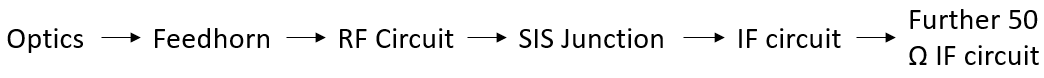
\includegraphics[width=0.9\textwidth]{./Images/Signal_Path.PNG}
	\caption{The path of the signal passes several stages where the RF circuit, the SIS junction and the IF circuit are located on the mixer chip.}
	\label{fig:Signal_Path}
\end{figure}

The RF circuit is designed to match the impedance of the feedhorn at the RF circuit's input and to match the impedance of the SIS junction at the RF circuit's output. The impedance of the SIS junction is non-linear and depends on its dimensions, its materials and its direct current (DC) bias. In the same way, the IF input is required to meet the SIS junctions output impedance. The IF circuit output is usually required to match 50\,\textOmega, which is the standard impedance for industrial products as amplifiers.

%Why is it important to know the embedding impedance?
%
%Designing Process
%
%Impedance Matching is necessary to match the impedances of different circuit elements to prevent reflections of the signal
%
%Single tone feed
%All elements can be represented by the Norton equivalent circuit

In general, any circuit can be replaced by a Norton equivalent circuit or Thevenin equivalent circuit. A Thevenin equivalent circuit consist of a voltage source and a series resistance, and the Norton equivalent circuit consist of a current source and a parallel resistance. 
This report uses the Norton equivalent circuit which is shown in figure \ref{fig:NortonEquivalentCircuit}. The telescope optics, feedhorn and RF circuit are represented by a current source and a parallel admittance, called embedded admittance. The SIS junction is represented by a parallel admittance. 
In the simplest case, the circuit is fed by a single frequency, the local oscillator signal (LO).
%For the following discussion, 
%The circuit is fed by a single tone signal, the local oscillator signal (LO).

\begin{figure}
	\centering
	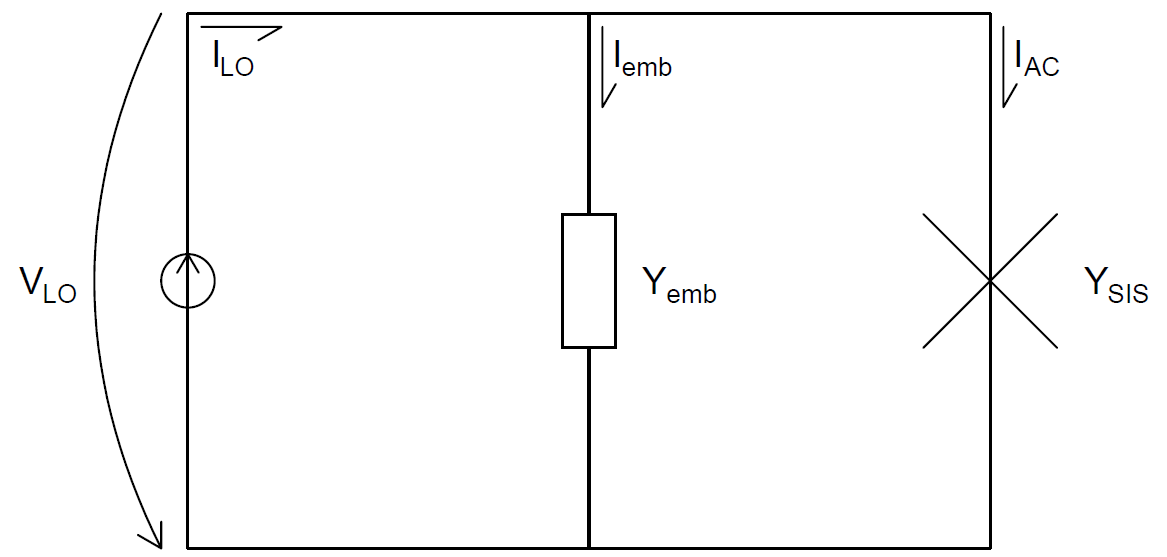
\includegraphics[width=0.7\textwidth]{./Images/Norton_Equivalent_Circuit.PNG}
	\caption{The Norton equivalent circuit of a Mixer chip has the embedding admittance parallel to the non-linear admittance of the SIS junction.}
	\label{fig:NortonEquivalentCircuit}
\end{figure}

From measurements of the DC current voltage (IV) response of the SIS junction, it is possible to recover the embedding admittance. The IV response forms so called photon steps as LO power is applied. The IV response without LO power is referred to as unpumped IV response, and the IV response with LO power applied is called pumped IV response. An example for an unpumped and pumped IV response is shown in  figure \ref{fig:Unpumped_Pumped}. These two DC responses are sufficient to compute the AC current and voltage of the SIS junction branch of the Norton equivalent circuit. Consequently, the admittance of the SIS junction can be computed  following the flowchart in figure \ref{fig:FlowchartSISJunctionBranch}. The admittance of the SIS junction is evaluated at every DC bias voltage to linearise the admittance, since the admittance of the SIS junction is intrinsically non-linear. Finally, the remaining characteristics of the Norton equivalent circuit can be computed knowing the AC characteristics of the SIS junction branch.

\begin{figure}
	\centering
	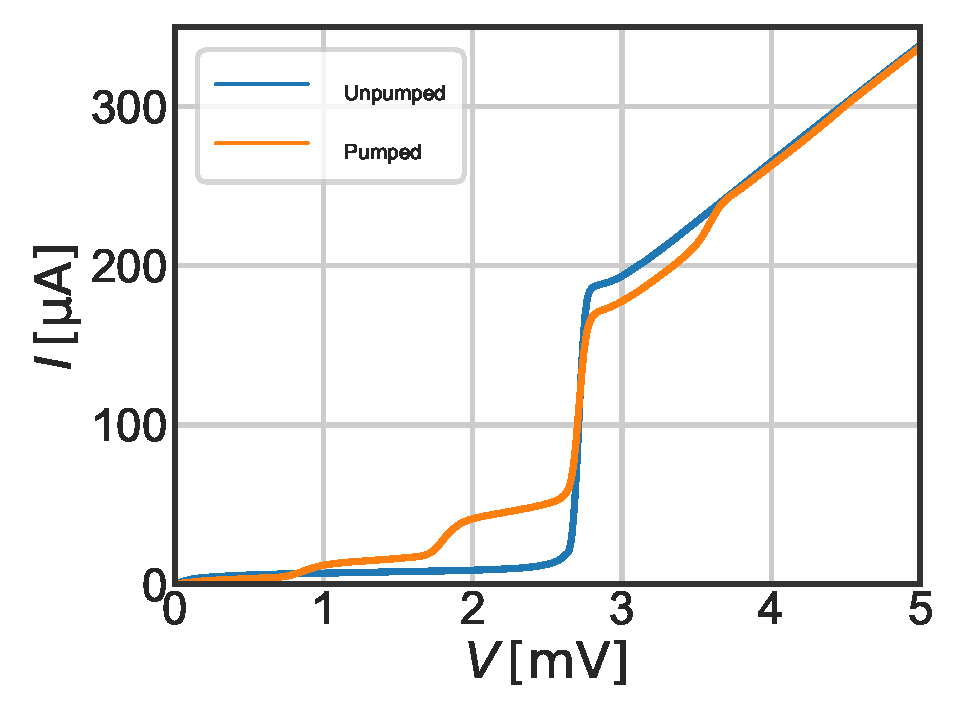
\includegraphics[width=0.7\textwidth]{./../Mixer_Unit_Test/2020_01_12_FixedMask/Unpumped_Pumped.pdf}
	\caption{The unpumped IV curve has no RF power applied, while the pumped IV curve is driven with an RF signal. }
	\label{fig:Unpumped_Pumped}
\end{figure}

\begin{figure}
	\centering
	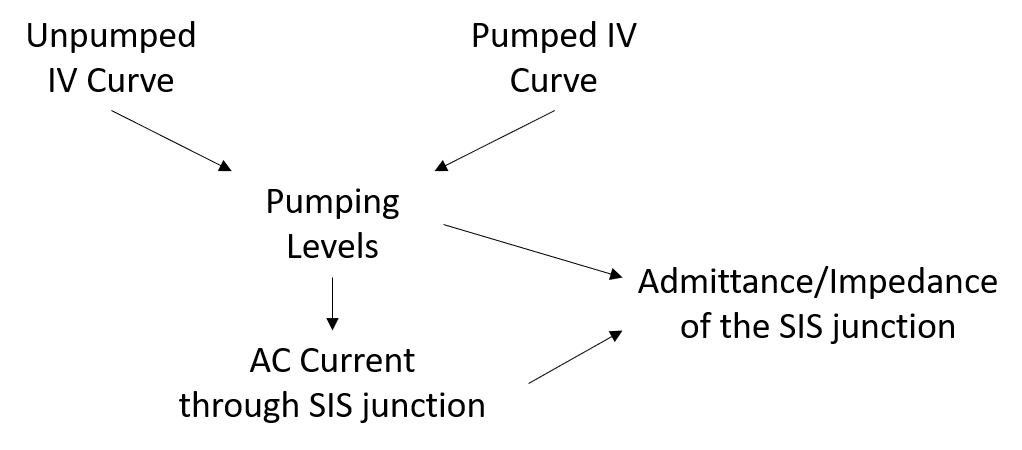
\includegraphics[width=0.7\textwidth]{./Images/Impedance_Recovery_Flowchart_Part1.png}
	\caption{The AC quantities of the SIS junction branch of the Norton equivalent circuit is determined following this flow chart.}
	\label{fig:FlowchartSISJunctionBranch}
\end{figure}

The following section describes the theory on which the admittance recovery is based. The method section describes the computation involved in the admittance recovery and how the theory is put into practise. Finally, the results are presented and discussed.

\section{Theory}
The theory of quasiparticle tunnelling in SIS junctions is described by \cite{Tucker1985}.
The unpumped and pumped DC IV response are connected by
\begin{equation}\label{eq:UnpumpedPumpedRelation}
I(V_0,V_\text{LO}) = \sum_{n=-\infty}^\infty J_n^2 (\alpha)\cdot I_0(V_0+n\cdot V_\text{Ph})
\end{equation}
where $I_0$ is the unpumped DC IV curve, $I$ is the pumped DC IV curve and $J_n$ is the $n^\text{th}$ order Bessel function of first kind evaluated at the normalised pumping level $\alpha = V_\text{LO}/V_\text{Ph}$. The photon voltage $V_\text{Ph}$ is given by the frequency $f_\text{LO}$ of the pump following
\begin{equation}\label{eq:PhotonVoltage}
	V_\text{Ph} = \frac{h\cdot f_\text{LO}}{e},
\end{equation} 
where $h$ is Planck's constant and $e$ is the electron charge.

The AC current through the SIS junction can be calculated knowing the pumping level. The real part is
\begin{equation}\label{eq:IacSIS_Re}
Re\{I_\text{AC}(V_0,V_\text{LO}) \}= \sum_{n=-\infty}^\infty J_n(\alpha)\cdot (J_{n-1}(\alpha)+J_{n+1}(\alpha))\cdot I_0(V_0+n\cdot V_\text{Ph}),
\end{equation}
and the imaginary part is 
\begin{equation}\label{eq:IacSIS_Im}
	Im\{I_\text{AC}(V_0,V_\text{LO}) \}= \sum_{n=-\infty}^\infty J_n(\alpha)\cdot (J_{n-1}(\alpha)-J_{n+1}(\alpha))\cdot I_\text{KK}(V_0+n\cdot V_\text{Ph}).
\end{equation}
$I_\text{KK}$ is the Kramers Kronig transformation of the unpumped IV curve $I_0$, a special case of the Hilbert transformation. 

Since the pumping level voltage and the AC current through the SIS junction are known, the admittance and impedance of the SIS junction can be computed as a linearisation of the junction at every bias voltage
\begin{equation}\label{eq:ySISLinearisation}
	 Y_\text{SIS}(V_0) = \frac{I_\text{AC}(V_0)}{V_\text{LO}(V_0)}~.
\end{equation}

The calculations above describe the branch of the SIS junction in the Norton equivalent circuit. The unknown quantities of the circuit, the current from the LO source $I_\text{LO}$, the current through the embedding admittance, and the embedding admittance $Y_\text{Emb}$, can be determined since the circuit equation 
\begin{equation}\label{eq:Circuit_Equation}
	I_\text{LO} - I_\text{AC}(V_0) =  V_\text{LO}(V_0)\cdot Y_\text{Emb}
\end{equation}
needs to hold for all bias voltages $V_0$. In fact, $I_\text{LO}$ is determined by 
\begin{equation}\label{eq:ILO_From_Circuit}
	I_\text{LO} = V_\text{LO}\cdot(Y_\text{Emb}+Y_\text{SIS})~.
\end{equation}
In consequence, the only unknown quantity of the Norton equivalent circuit is the embedding admittance.


\section{Methods}

Data from the unpumped and pumped IV curves is necessary to perform the admittance recovery. The computation of a single IV response and the computation of the interaction of the IV responses can be separated. The computation of a single IV dataset is described in the following IV Response section \ref{sec:IVResponse}. In the Mixer section \ref{sec:Mixer}, the computation of the admittance recovery is described. Both, the IV Response section and the Mixer section, correspond to separate classes coded in Python.

\subsection{IV Response} \label{sec:IVResponse}
\subsubsection{Data Handling}
The \texttt{IV\_Response} class handles a single IV dataset. Experimentally, these datasets are obtained by sweeping the voltage up and down to conserve hysteresis behaviour. The voltage sweeping limits, the number of data points and a few other parameters depending on the experimental setup are controlled with a Labview readout program. The program stores data in \texttt{.csv} files. The \texttt{IV\_Response} class reads the dataset from a location defined by the user.\footnote{There are keyword arguments (\texttt{headerLines}, \texttt{footerLines}, \texttt{columnOffset}) to specify the layout of the \texttt{.csv} file. The only requirement is that the file contains a column with voltage data stored next to current data. The unit of the current data can be specified with the keyword argument \texttt{currentFactorToMicroampere}.} The current data sorted by their index in figure \ref{fig:rawDatabyTime} shows the sweep behaviour.

\begin{figure}
	\centering
	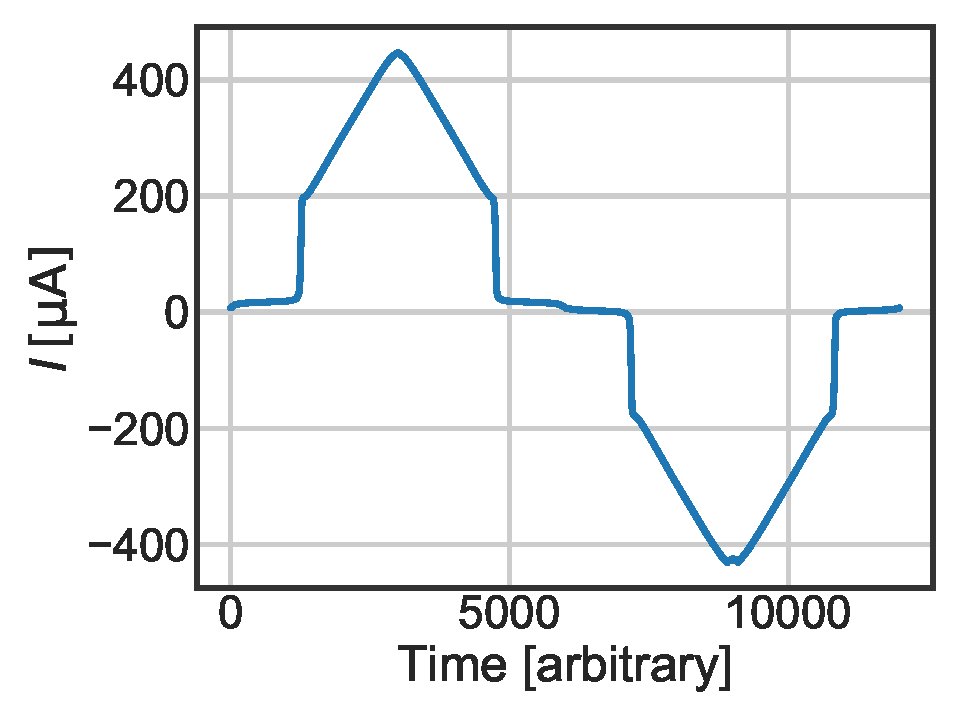
\includegraphics[width=0.7\textwidth]{./../IV_Class_Unit_Test/2020_01_14/Raw_Data_by_Time.pdf}
	\caption{The IV data is recorded by sweeping the voltage up and down, starting close to 0\,V. The time axis shows the indexes of the IV entries in the \texttt{.csv} file.}
	\label{fig:rawDatabyTime}
\end{figure}

The first data processing step is the correction of the current and voltage offset.\footnote{The offset correction can be skipped by entering the offset in the keyword argument \texttt{fixedOffset}.} At the origin, the IV curve shows a larger slope than in the remaining subgap region as shown in figure \ref{fig:rawDataSlopebyVoltage}. For this reason, the slope of the raw data is computed. The largest two slopes originate from the sweep with positive and negative voltage gradient.\footnote{The voltage offset is searched within a voltage range determined by the keyword argument \texttt{offsetThreshold}.} The voltages of the peaks are averaged and interpreted as voltage offset. The current offset is determined from the average of the currents at the two voltage values in the IV dataset closest to the voltage offset.

\begin{figure}
	\centering              
	\begin{subfigure}[t]{0.49\textwidth}
		\centering
		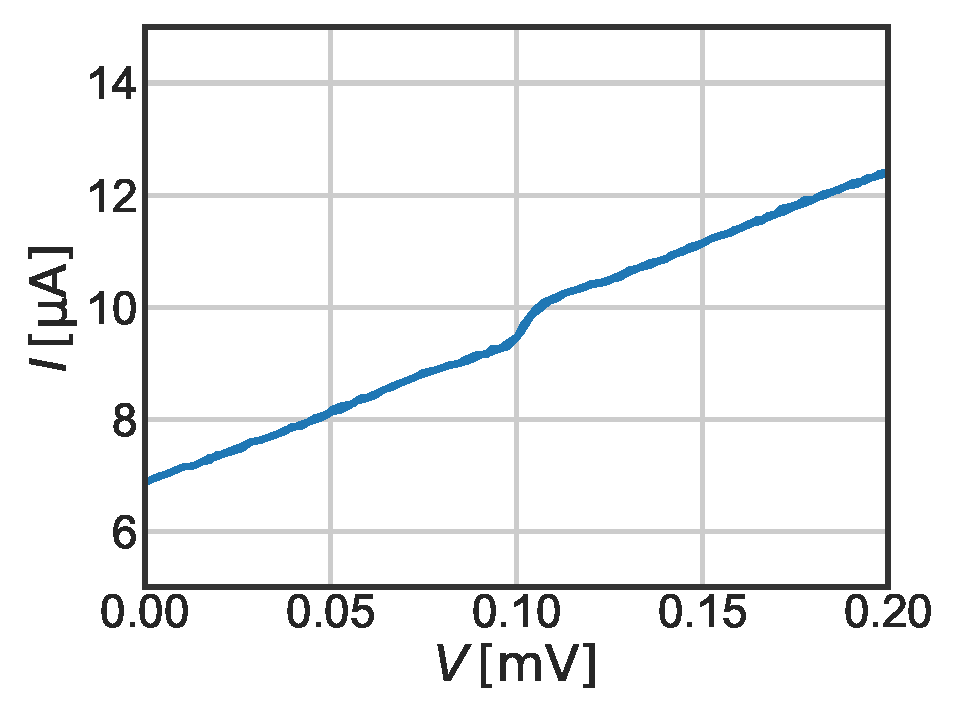
\includegraphics[width=\linewidth]{./../IV_Class_Unit_Test/2020_01_14/Raw_Data_at_Origin.pdf}
		\caption{At the true origin, the IV curve shows a transition between negative and positive subgap current. The transition has a slightly larger slope. }
	\end{subfigure}
	\begin{subfigure}[t]{0.49\textwidth}
		\centering
		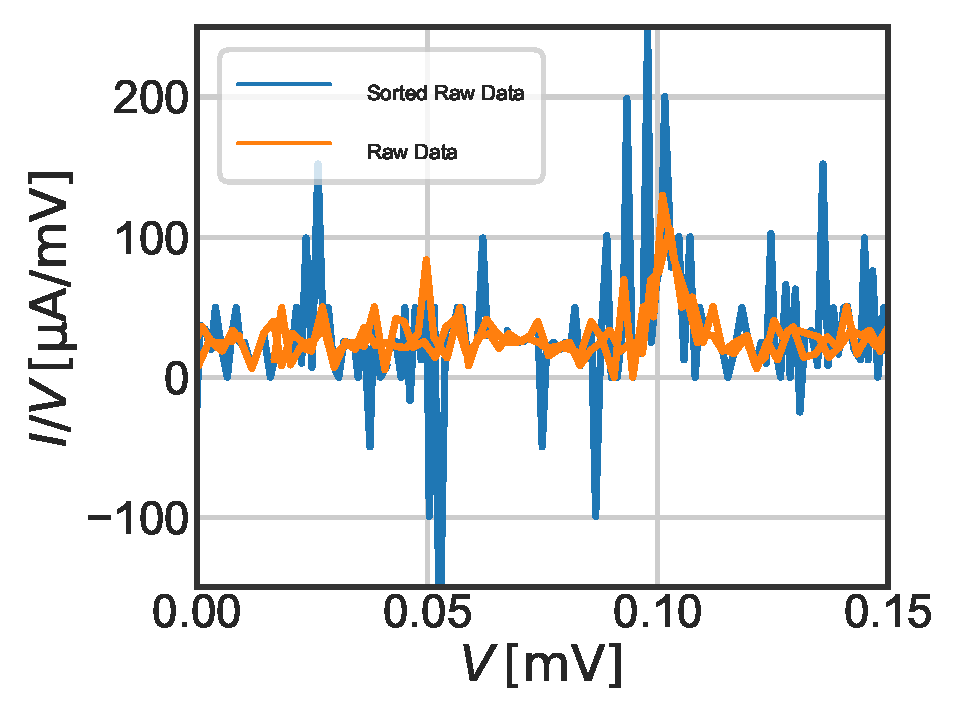
\includegraphics[width=\linewidth]{./../IV_Class_Unit_Test/2020_01_14/Sorted_vs_Unsorted_Slope.pdf}
		\caption{The offset can be found as peaks in the slope between the data points of the raw dataset, which contains the sweep in positive and negative voltage direction. Sorting the dataset by increasing voltage introduces artificial peaks in the slope. For this reason, the offset is determined from the unmodified `raw' IV dataset.}
	\end{subfigure}
	\caption[]{The recorded IV dataset shows an offset in voltage and current.
	}
	\label{fig:rawDataSlopebyVoltage}
\end{figure}

Subsequently, the dataset is sorted by increasing voltage. The slope of the sorted dataset is distorted as shown in figure \ref{fig:rawDataSlopebyVoltage} and is therefore not suitable for offset determination. The effect on the path of the IV curve at the transition is shown in figure \ref{fig:Sorted_vs_Unsorted_vs_Filtered_Raw_Data}. The sorted dataset is smoothed with a Savitzky-Golay filter to average the hysteresis behaviour.\footnote{The Savitzky-Golay filter is part of the \texttt{scipy.signal} package. Its parameters are accessible via the keyword arguments \texttt{savgolWindow} and \texttt{savgolOrder}. }
\begin{figure}
	\centering
	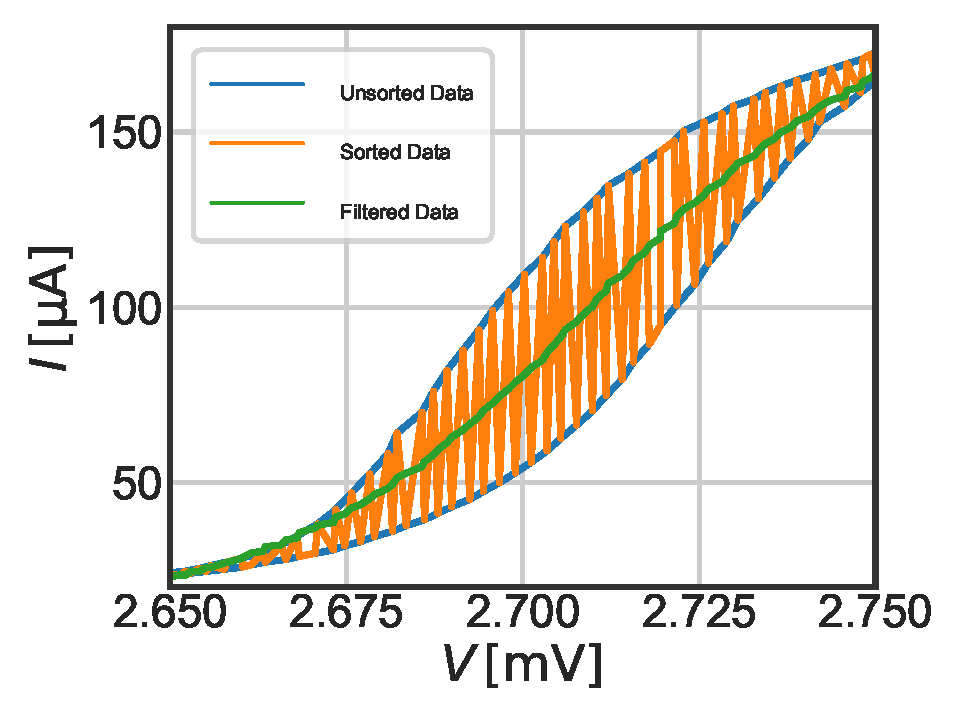
\includegraphics[width=0.7\textwidth]{./../IV_Class_Unit_Test/2020_01_14/Sorted_vs_Unsorted_vs_Filtered_Raw_Data.pdf}
	\caption{The data is recorded by sweeping the voltage up and down to include hysteresis behaviour. Sorting the dataset after increasing voltage leads to rapid fluctuations of the IV curve, especially at the transition. This sorted dataset is filtered with Savitzky-Golay filter to obtain a smooth IV curve representing an average of the hysteresis.}
	\label{fig:Sorted_vs_Unsorted_vs_Filtered_Raw_Data}
\end{figure}

The filtered data is then allocated in equispaced voltage bins to avoid complications at later stages, especially in dealing with both the unpumped and pumped IV curves.\footnote{The parameters for binning the data are interfered by the keyword arguments \texttt{numberOfBins}, \texttt{vmin} and \texttt{vmax}.} The effect of binning the filtered data instead of the voltage sorted dataset is shown in figure \ref{fig:Filtered_Binning_Impact_Raw_Data}.

\begin{figure}
	\centering
	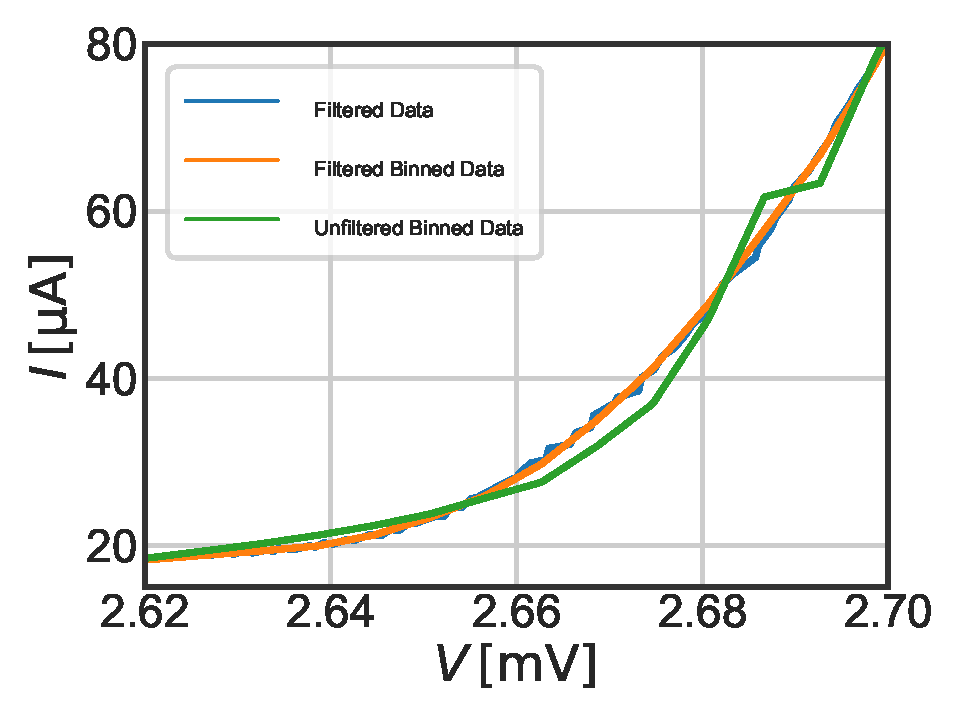
\includegraphics[width=0.7\textwidth]{./../IV_Class_Unit_Test/2020_01_14/Filtered_Binning_Impact_Raw_Data.pdf}
	\caption{The Savitzky-Golay filtered IV curve shows some minor fluctuations. The filtered dataset is binned into equispaced voltage bins to smoothen these fluctuations and to obtain an equispaced voltage axis. Binning of the unfiltered data leads to artificial steps in the IV response. }
	\label{fig:Filtered_Binning_Impact_Raw_Data}
\end{figure}

\subsubsection{Determination of Characteristic Values}
The characteristic values of the IV response are determined after processing the dataset. The normal and subgap resistance are determined through linear regression of the offset corrected raw data sorted by increasing voltage within the corresponding voltage ranges.\footnote{The voltage ranges used for the linear regression are adjustable by the keyword arguments \texttt{rNThresholds} and \texttt{rSGThresholds}} Separate fits through the negative and positive bias regime are performed, then averaged. The errors of the linear regressions are propagated to an error of the normal and subgap resistance respectively. The linear regressions are shown in figure \ref{fig:ResistanceLinearRegression}.

\begin{figure}
	\centering              
	\begin{subfigure}[t]{0.49\textwidth}
		\centering
		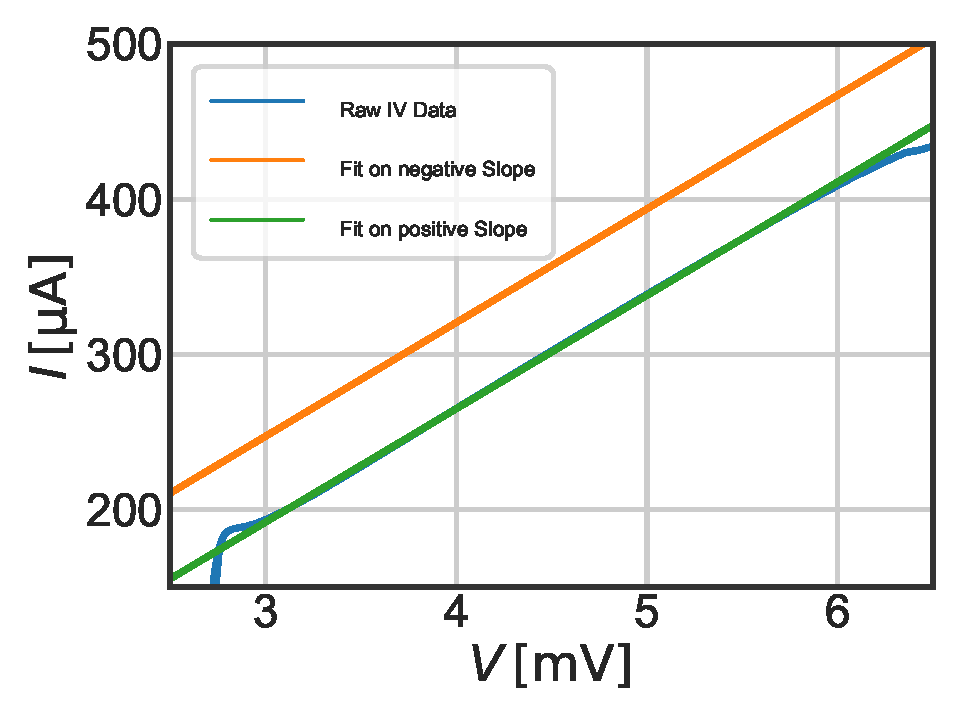
\includegraphics[width=\linewidth]{./../IV_Class_Unit_Test/2020_01_14/Normal_Resistance_Fit.pdf}
		\caption{The linear regression through the normal resistance regime.}
	\end{subfigure}
	\begin{subfigure}[t]{0.49\textwidth}
		\centering
		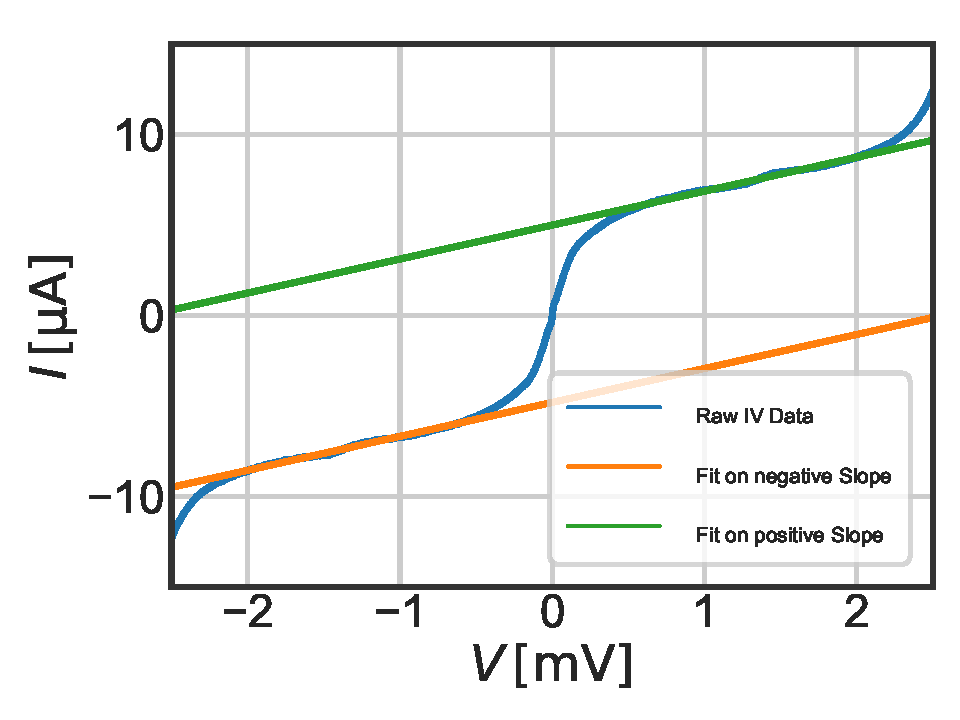
\includegraphics[width=\linewidth]{./../IV_Class_Unit_Test/2020_01_14/Subgap_Resistance_Fit.pdf}
		\caption{The linear regression through the subgap resistance regime.}
	\end{subfigure}
	\caption[]{The linear regressions are performed separately for negative and positive bias voltages.
	}
	\label{fig:ResistanceLinearRegression}
\end{figure}

The gap voltage is determined from the maximum slope of the binned IV data at the transition voltage regime.\footnote{The voltage regime evaluated for the determination of the gap voltage is accessible via the keyword argument \texttt{vGapSearchRange}.} Figure \ref{fig:Filtered_Binning_Impact_Raw_Data} shows negligible fluctuations in the binned IV dataset in comparison to the Savitzky-Golay filtered dataset. The effect on the slope is shown in figure \ref{fig:Filtered_Binning_Impact_Slope_Transission}. The maximum slopes at negative and positive bias voltages are averaged to obtain the gap voltage.\footnote{A suggested improvement would involve the fit of a gaussian on the transition and using its peak as gap voltage. However, this would be accompanied by a computationally more intense fitting. } 

\begin{figure}
	\centering
	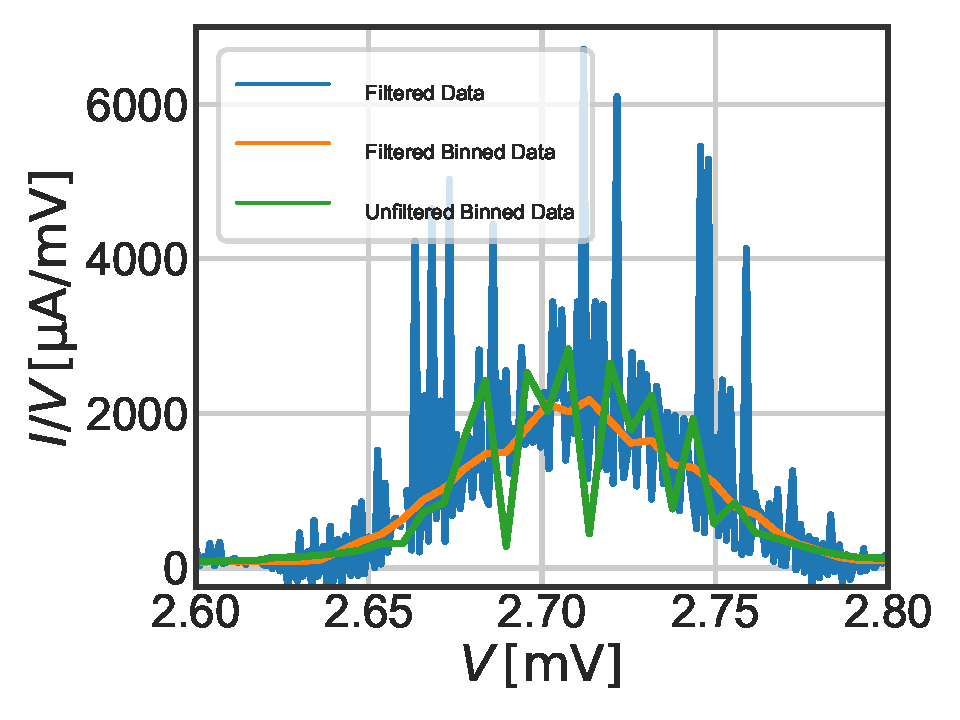
\includegraphics[width=0.7\textwidth]{./../IV_Class_Unit_Test/2020_01_14/Filtered_Binning_Impact_Slope_Transission.pdf}
	\caption{The maximum slope at the transition is used to determine the gap voltage. The Savgol-Golay filtered dataset and the unfiltered dataset show strong fluctuations. Binning of the Savgol-Golay filtered dataset leads to a smooth IV response and minimum fluctuations in its slope.}
	\label{fig:Filtered_Binning_Impact_Slope_Transission}
\end{figure}

The critical current is determined from the normal resistance and the gap voltage as
\begin{equation}
	I_\text{C} = \frac{V_\text{gap}}{R_\text{N}},
\end{equation}
where $V_\text{gap}$ is the gap voltage and $R_\text{N}$ is the normal resistance. 
Alternatively, the critical current can be determined from the current after the transition. Liu et al. [2017] described the critical current as
\begin{equation}
I_\text{C} = I_\text{gap}\cdot\frac{\pi}{4},
\end{equation}
where $I_\text{gap}$ is the current after the transition. This current is determined by the first negative slope in the binned IV data after the gap voltage.

\subsubsection{Simulated IV Response}
The characteristic values determine an IV response. For calculations involving certain portions of the IV curve, a simulated IV response with a larger number of data points can be convenient. In that case, the IV response is described by a model with certain parameters instead of the IV curve's characteristic values. The \texttt{IV\_Response} class has several models implemented. The currently implemented methods are based on two approaches, namely the Chalmers approach and the gaussian convolution approach.

The Chalmers approach uses the equation 
\begin{equation}
\begin{split}
	I(V) = &~~ \frac{V}{R_\text{SG}}\cdot\left(1+\text{e}^{-a\cdot(V+V_\text{gap})}\right)^{-1}
	+\frac{V}{R_\text{N}}\cdot\left(1+\text{e}^{a\cdot(V+V_\text{gap})}\right)^{-1}
	\\&+\frac{V}{R_\text{SG}}\cdot\left(1+\text{e}^{a\cdot(V-V_\text{gap})}\right)^{-1}
	+\frac{V}{R_\text{N}}\cdot\left(1+\text{e}^{-a\cdot(V-V_\text{gap})}\right)^{-1}
\end{split}
\end{equation}
presented by \cite{Rashid2016} with the fitting parameter $a$. The fit shown in figure \ref{fig:Chalmers} shows good agreement in describing the transition, but bad fitting of the subgap regime.

\begin{figure}
	\centering              
	\begin{subfigure}[t]{0.49\textwidth}
		\centering
		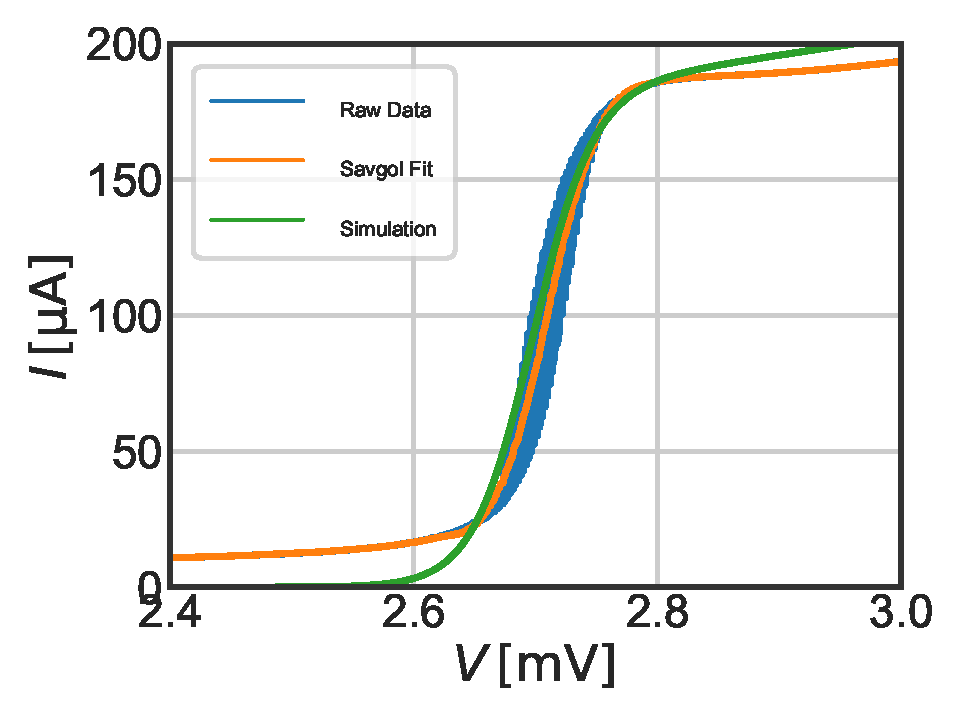
\includegraphics[width=\linewidth]{./../IV_Class_Unit_Test/2020_01_14/Simulation_Chalmers_Transission.pdf}
	\end{subfigure}
	\begin{subfigure}[t]{0.49\textwidth}
		\centering
		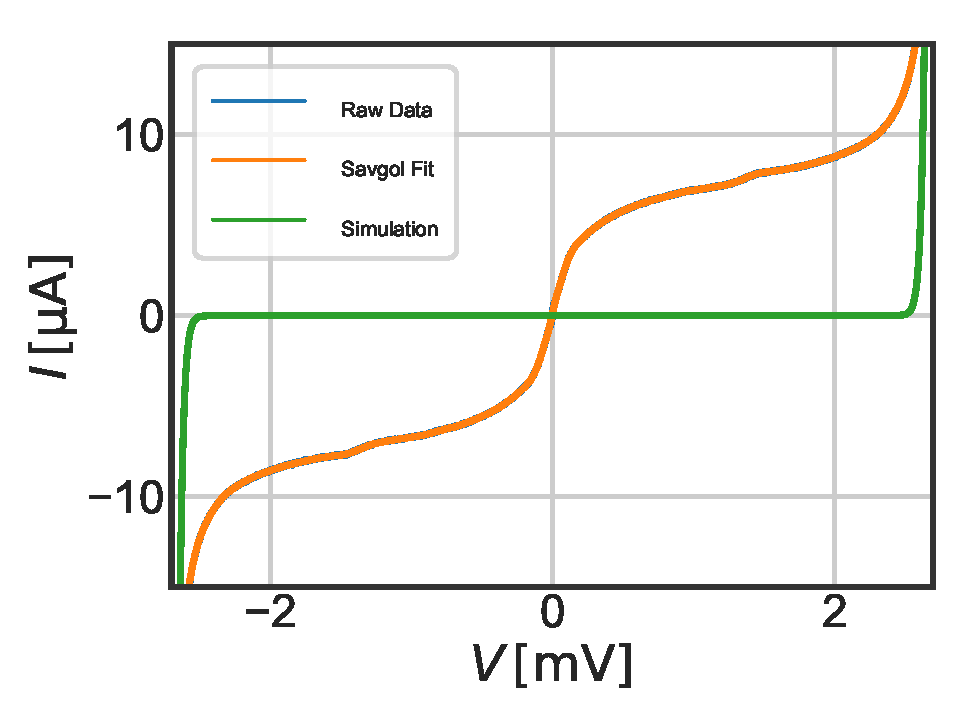
\includegraphics[width=\linewidth]{./../IV_Class_Unit_Test/2020_01_14/Simulation_Chalmers_Subgap.pdf}
	\end{subfigure}
	\caption[]{The Chalmer approach leads to good agreement with the data in the transition region. In the subgap region, however, the simulation agrees badly with the data.
	}
	\label{fig:Chalmers}
\end{figure}

The gaussian convolution method is implemented for a better description of the subgap resistance. The idea of this method is to convolve a perfect IV curve with a gaussian of a certain width. The parameters of this model involve the width of the gaussian and the parameters of the IV curve. The simplest IV curve has no subgap leakage, a step function at the transition and a normal resistance slope afterwards as shown in figure \ref{fig:Perfect}. A subgap current can be included by a constant non-zero value in the subgap region as shown in figure \ref{fig:SubgapLeakageOffset}. The constant corresponds to a step function at 0\,V. An even better agreement of the model with the data is achieved by including a subgap resistance slope as shown in figure \ref{fig:SubgapLeakage_SubgapLeakageOffset}. Finally, efforts in optimising the description of regions just before and after the transition led to include an excess current at the transition to the model, shown in figure \ref{fig:ExcessCriticalCurrent_SubgapLeakage_and_SubgapLeakageOffset}.

\begin{figure}
	\centering
	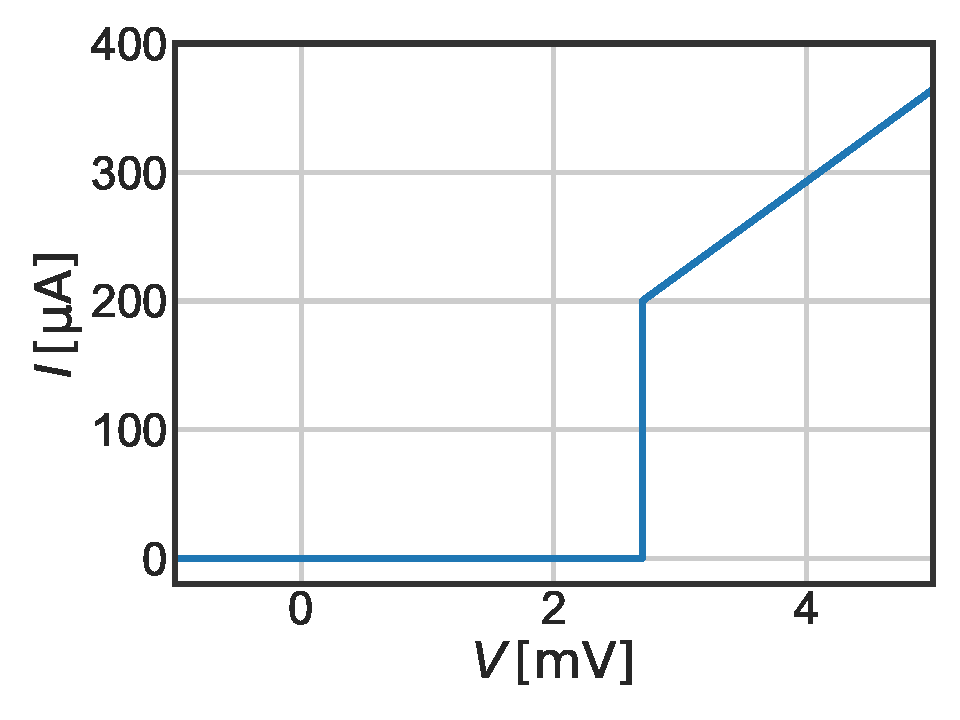
\includegraphics[width=0.7\textwidth]{./../IV_Curve_Simulations_Unit_Test/2020_01_06//Perfect.pdf}
	\caption{The model of a perfect IV reponse has no subgap current and a step function at the gap voltage followed by a normal resistance slope.}
	\label{fig:Perfect}
\end{figure}
\begin{figure}
	\centering
	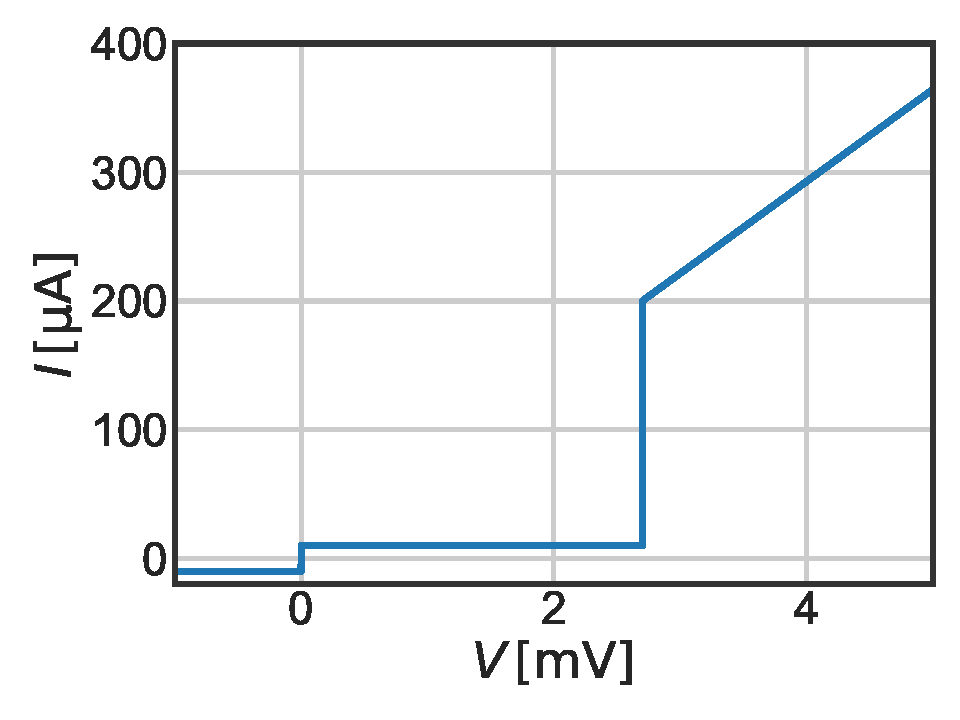
\includegraphics[width=0.7\textwidth]{./../IV_Curve_Simulations_Unit_Test/2020_01_06//SubgapLeakageOffset.pdf}
	\caption{The model of a perfect IV curve can be expanded by including a finite constant subgap current.}
	\label{fig:SubgapLeakageOffset}
\end{figure}
\begin{figure}
\centering
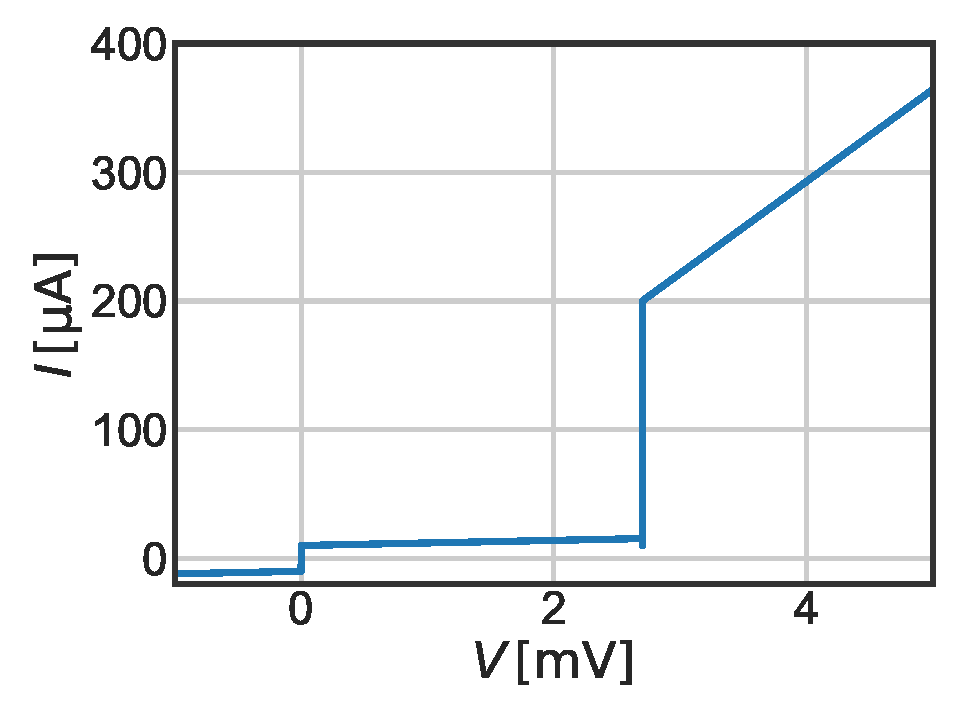
\includegraphics[width=0.7\textwidth]{./../IV_Curve_Simulations_Unit_Test/2020_01_06//SubgapLeakage_SubgapLeakageOffset.pdf}
\caption{The subgap region of a perfect IV curve can be modelled with a subgap resistance and a step function at the origin.}
\label{fig:SubgapLeakage_SubgapLeakageOffset}
\end{figure}
\begin{figure}
\centering
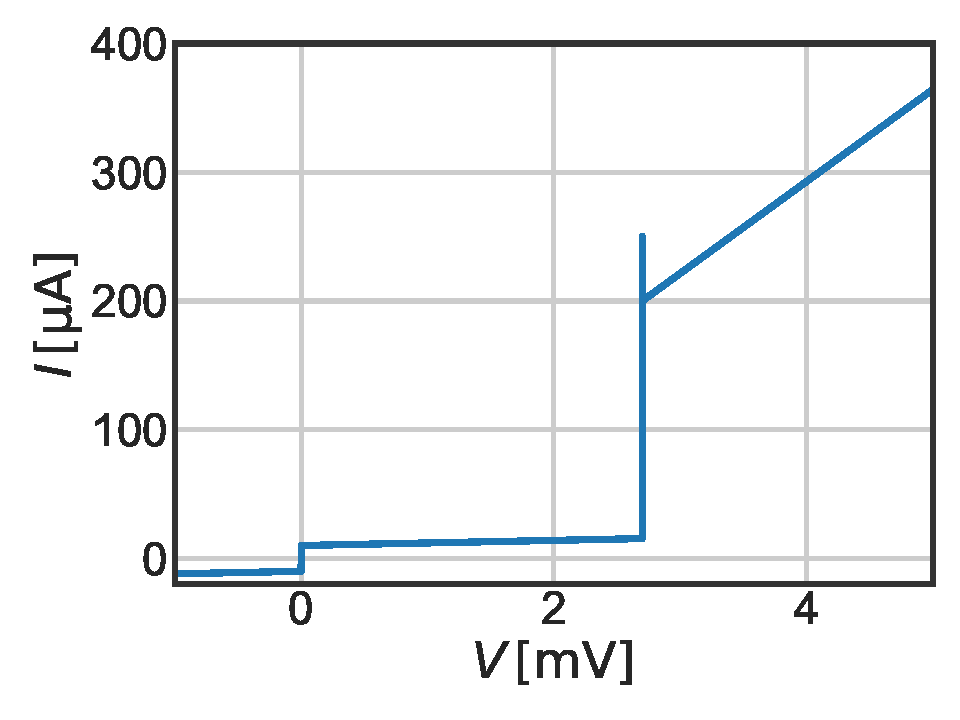
\includegraphics[width=0.7\textwidth]{./../IV_Curve_Simulations_Unit_Test/2020_01_06//ExcessCriticalCurrent_SubgapLeakage_and_SubgapLeakageOffset.pdf}
\caption{The perfect IV curve model with subgap current simulation can be expanded by a excess current at the transition, to improve the fit at bias voltages close to the transition after the convolution with a gaussian. }
\label{fig:ExcessCriticalCurrent_SubgapLeakage_and_SubgapLeakageOffset}
\end{figure}

There are different methods implemented to fit the presented models convolved with a gaussian to the Savitzky-Golay filtered data. Best performance is achieved with a stepwise fit, where the parameters are adjusted at the voltage regime they have most impact on. For example, the subgap leakage parameters are fitted in the same region as the subgap resistance is determined. The simulation and the Savitzky-Golay filtered data are shown in figure \ref{fig:Simulation_Stepwise}.\par

\begin{figure}
	\centering              
	\begin{subfigure}[t]{0.49\textwidth}
		\centering
		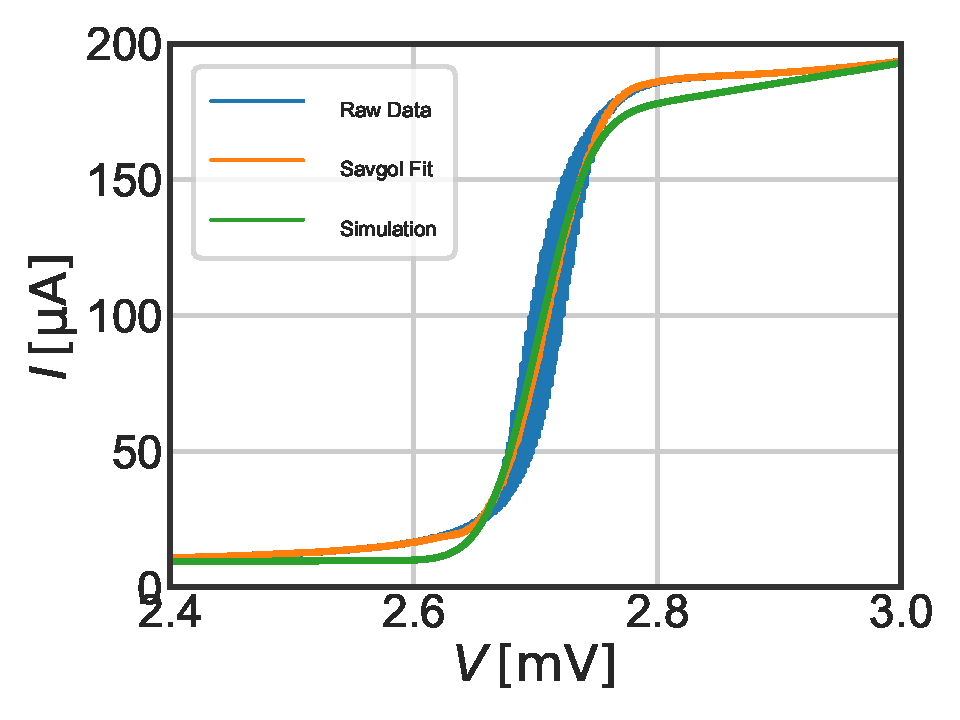
\includegraphics[width=\linewidth]{./../IV_Class_Unit_Test/2020_01_14/Simulation_Stepwise_Transission.pdf}
	\end{subfigure}
	\begin{subfigure}[t]{0.49\textwidth}
		\centering
		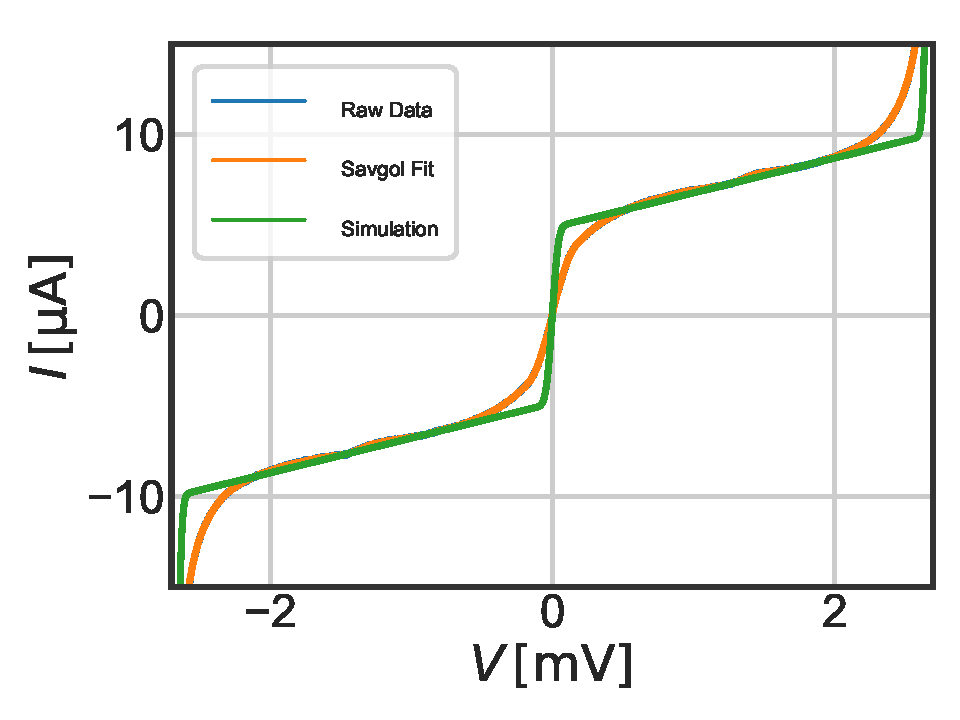
\includegraphics[width=\linewidth]{./../IV_Class_Unit_Test/2020_01_14/Simulation_Stepwise_Subgap.pdf}
	\end{subfigure}
	\caption[]{The convolution of a gaussian with an IV curve with subgap current offset, subgap resistance and an excess current at the transition leads to good agreement with the data. 
	}
	\label{fig:Simulation_Stepwise}
\end{figure}

\subsection{Mixer}\label{sec:Mixer}
The unpumped and pumped IV responses are used to determine the embedding admittance of the mixer. The \texttt{Mixer} class connects the \texttt{IV\_Response} objects of the unpumped and pumped IV datasets to perform this calculation.\footnote{The unpumped and pumped \texttt{IV\_Response} objects are the \texttt{Unpumped} and \texttt{Pumped} arguments in the \texttt{Mixer} object.}

\subsubsection{AC Characteristic of the SIS Junction Branch}
In the first step, equation \ref{eq:UnpumpedPumpedRelation} is used to evaluate the pumping level at all bias voltages $V_0$. Consequently, the pumping level is a function of the bias voltage $\alpha(V_0)$ as shown in figure \ref{fig:Pumping_Level}. This calculation requires the unpumped IV curve to be evaluated at bias voltages $V_0+n\cdot V_\text{Ph}$, where $n$ runs in theory from $-\infty$ to $+\infty$. The photon voltage is determined from the pumping frequency $f_\text{LO}$ following equation \ref{eq:PhotonVoltage}.\footnote{The pumping frequency $f_\text{LO}$ is given by the keyword argument \texttt{fLO}.} In fact, $n$ is limited to a finite value for effective computation, since the multiplicative value of the Bessel function $J_n$ vanishes at larger values of $n$.\footnote{The summation index is accessible via the keyword argument \texttt{tuckerSummationIndex}.} The unpumped IV curve data needs to be expanded to larger voltages to be able to evaluate the unpumped data at $V_0+n\cdot V_\text{Ph}$. This is done with the information of the junctions normal resistance. Likewise, the Kramers Kronig transformation of the unpumped IV curve uses this expanded voltage regime.\footnote{The expansion and Kramers Kronig transformation is done within the \texttt{IV\_Response} object of the unpumped IV data.}

\begin{figure}
	\centering
	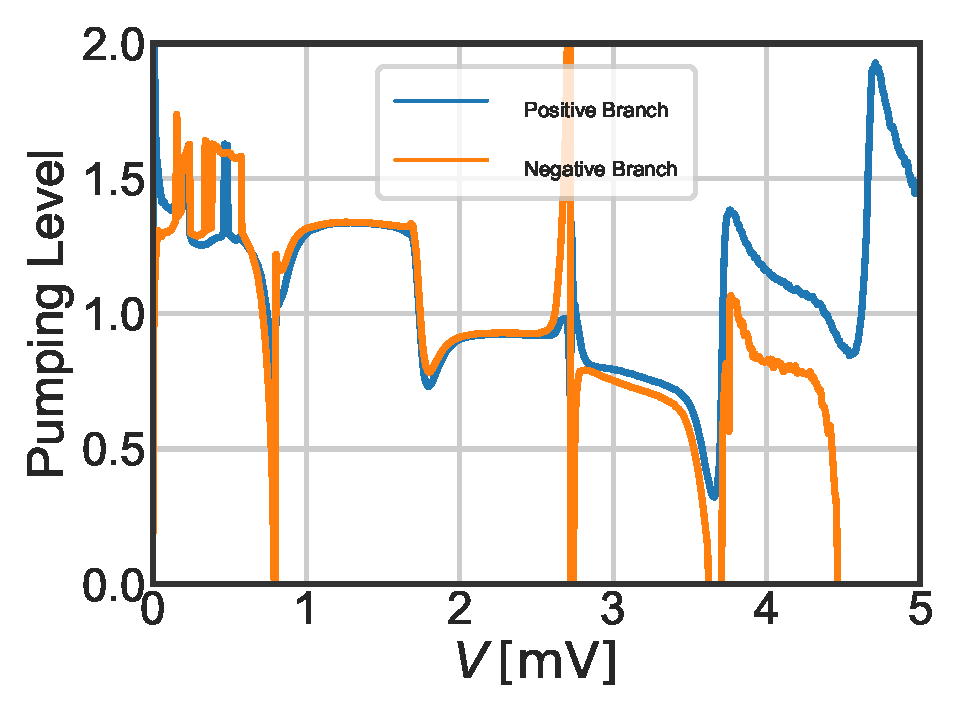
\includegraphics[width=0.7\textwidth]{./../Mixer_Unit_Test/2020_01_12_FixedMask/Pumping_Level.pdf}
	\caption{The pumping level is evaluated from the unpumped and pumped IV response at every single bias voltage. The pumping level from negative bias voltages is close to the pumping level of the corresponding positive bias voltages.}
	\label{fig:Pumping_Level}
\end{figure}

The expanded unpumped IV curve and the corresponding Kramers Kronig transformation in conjunction with the pumping level are used to compute the AC current through the SIS junction following equation \ref{eq:IacSIS_Re} and \ref{eq:IacSIS_Im}.\footnote{The methods \texttt{iACSISRe\_Calc} and \texttt{iACSISIm\_Calc} are used to compute the arguments \texttt{iACSISRe} and \texttt{iACSISIm}. The results are concatenated to the complex AC current \texttt{iACSIS}.} The AC current  through the SIS junction, evaluated at every bias voltage, is shown in figure \ref{fig:iACSIS}.

\begin{figure}
	\centering
	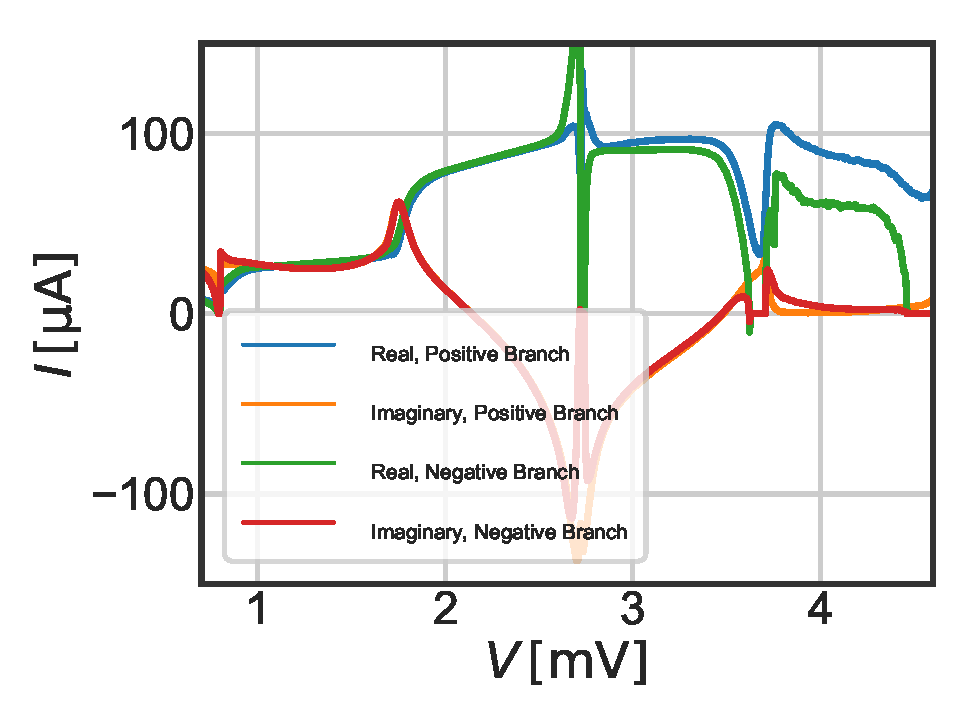
\includegraphics[width=0.7\textwidth]{./../Mixer_Unit_Test/2020_01_12_FixedMask/Current_through_Junction.pdf}
	\caption{The real and imaginary AC current are calculated from the pumping level at every bias voltage. Both negative and positive bias voltages are displayed.}
	\label{fig:iACSIS}
\end{figure}

The admittance of the SIS junction can be linearised for every bias voltage following equation \ref{eq:ySISLinearisation}. The admittance and the impedance, which is the reciprocal of the admittance, are shown in figure \ref{fig:ySIS}.

\begin{figure}
	\centering              
	\begin{subfigure}[t]{0.49\textwidth}
		\centering
		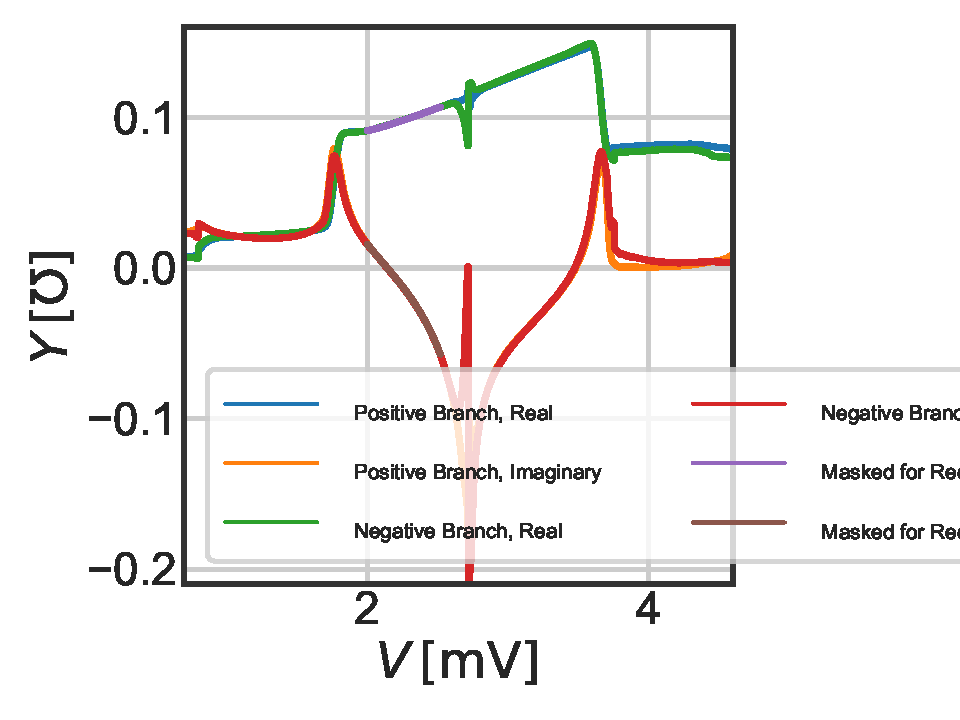
\includegraphics[width=\linewidth]{./../Mixer_Unit_Test/2020_01_12_FixedMask/Admittance_Junction.pdf}
	\end{subfigure}
	\begin{subfigure}[t]{0.49\textwidth}
		\centering
		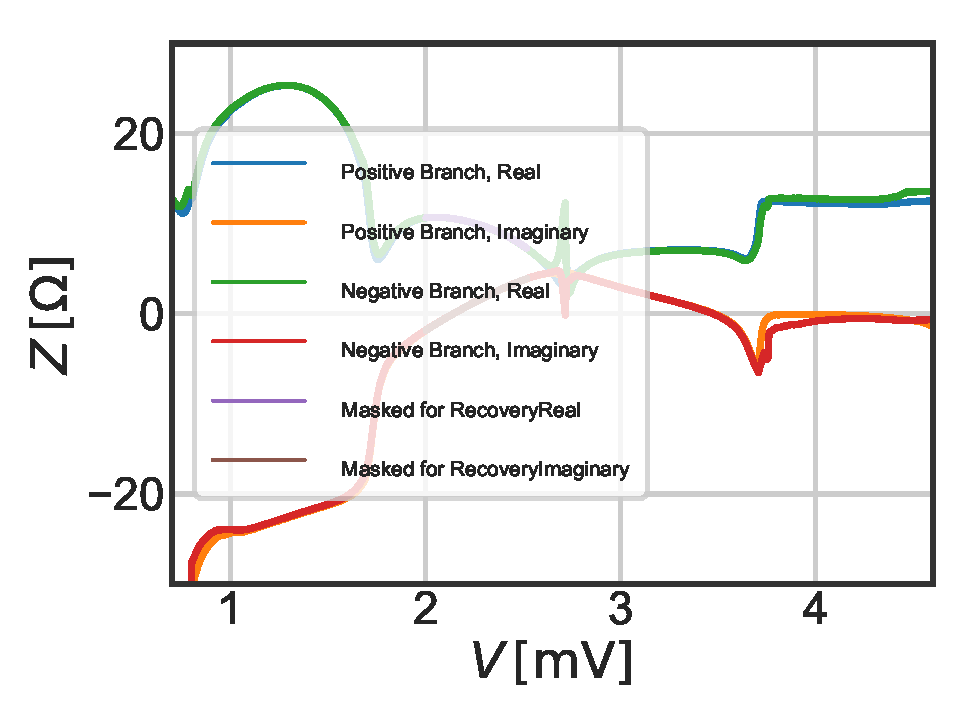
\includegraphics[width=\linewidth]{./../Mixer_Unit_Test/2020_01_12_FixedMask/Impedance_Junction.pdf}
	\end{subfigure}
	\caption[]{The embedding admittance and impedance show an almost linear response at the first photon step.
	}
	\label{fig:ySIS}
\end{figure}

\subsubsection{Embedding Admittance Recovery}
The embedding admittance is computed from the first photon steps of the quantities computed above.\footnote{The number of photon steps involved is determined by the keyword argument \texttt{steps\_ImpedanceRecovery}.} The width of the photon step is $V_\text{Ph}$, and the photon steps are counted from the gap voltage into the subgap region. Figure \ref{fig:Masked_Photon_Steps} shows the two masking strategies applied on the first photon step.\footnote{The used masking strategy and its parameters are accessible via the keyword argument \texttt{maskingWidth}.} In general, parts close to the boundary of the photon step are excluded from processing, since there is a transition between the single photon steps and the transition of the IV curve itself. These effects arise from the fact that the tunnelling of quasiparticles through the SIS junction is a probability function. The first masking strategy excludes a certain voltage range at the boundary of the photon step, similar to the QMix package. The second masking strategy fits the slope of the transition of the IV curve with a gaussian as shown in figure \ref{fig:Gaussian_Fit_on_Positive_Slope}. The masked voltage range is the photon step width reduced by four times the width of this gaussian fit on each side.

\begin{figure}
	\centering              
	\begin{subfigure}[t]{0.49\textwidth}
		\centering
		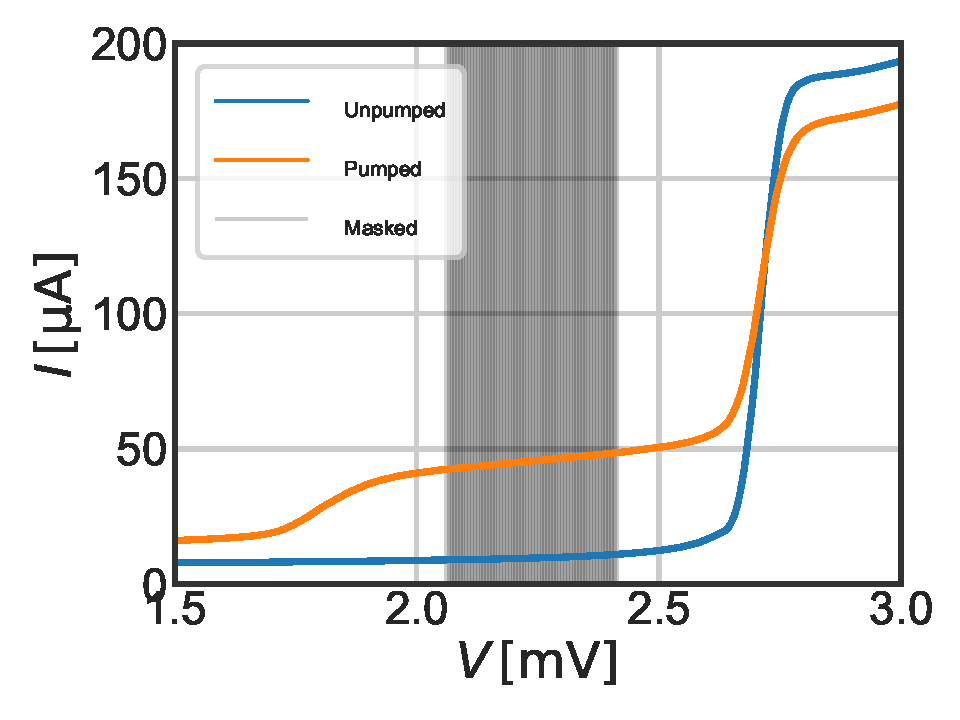
\includegraphics[width=\linewidth]{./../Mixer_Unit_Test/2020_01_12_GausMask/Masked_Voltage_Region.pdf}
		\caption{This method uses a gaussian fit on the transition of the IV curve.}
	\end{subfigure}
	\begin{subfigure}[t]{0.49\textwidth}
		\centering
		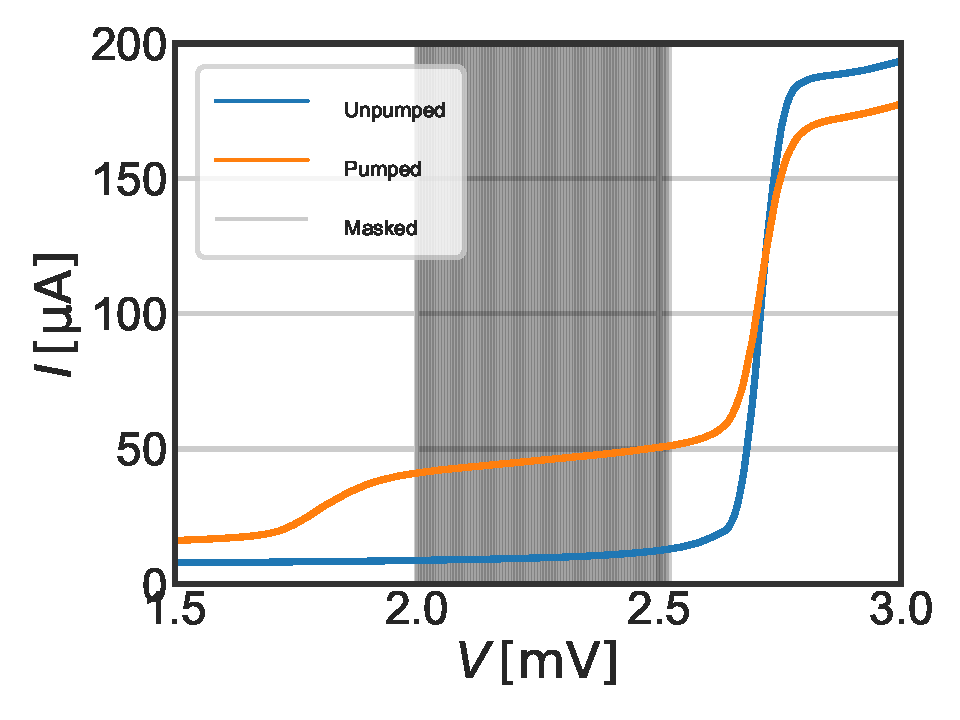
\includegraphics[width=\linewidth]{./../Mixer_Unit_Test/2020_01_12_FixedMask/Masked_Voltage_Region.pdf}
		\caption{This method uses boundaries defined by the user.}
	\end{subfigure}
	\caption[]{The bias voltages of the first photon step used for the admittance recovery can be selected using two methods.
	}
	\label{fig:Masked_Photon_Steps}
\end{figure}

\begin{figure}
	\centering
	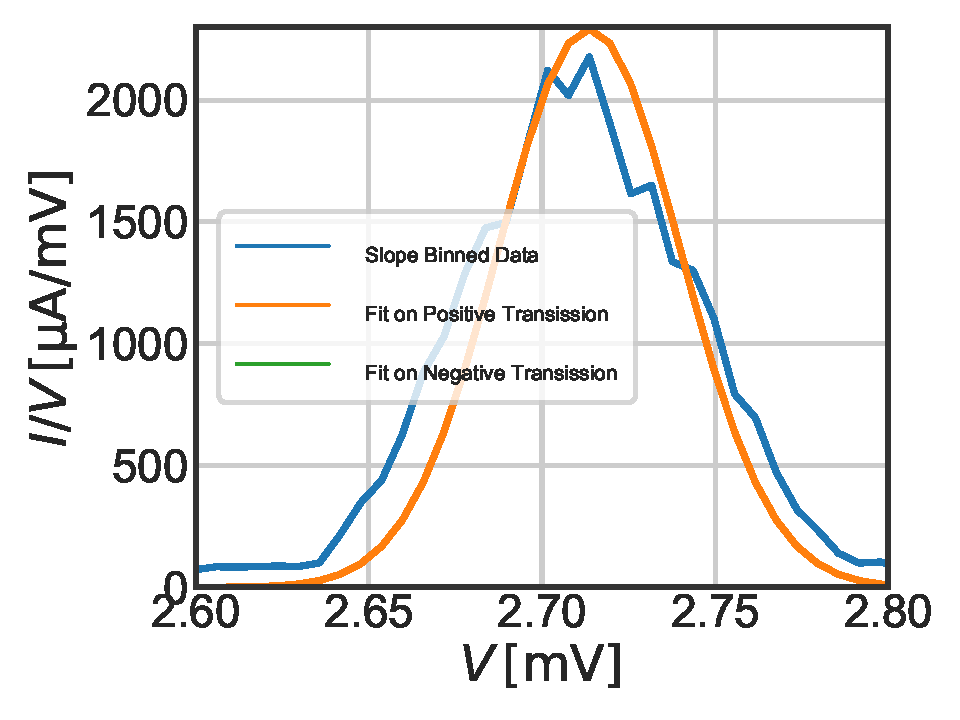
\includegraphics[width=0.7\textwidth]{./../IV_Class_Unit_Test/2020_01_14/Gaussian_Fit_on_Positive_Slope.pdf}
	\caption{The slope of the transition is fitted with a gaussian. The width of the gaussian is used for one of the masking methods.}
	\label{fig:Gaussian_Fit_on_Positive_Slope}
\end{figure}

The embedding admittance is then recovered using the masked quantities of the SIS junctions branch in the Norton equivalent circuit. This is possible since the circuit equation \ref{eq:Circuit_Equation} needs to hold for all bias voltages $V_0$. The problem becomes a minimisation problem since the data is noisy. The class contains different cost functions associated with the minimisation problem, but they lead to similar result. In general, there are two kinds of cost functions, those with the $I_\text{LO}$ as a parameter and those which compute $I_\text{LO}$ from the embedding admittance using equation \ref{eq:ILO_From_Circuit}.\footnote{Both methods are implemented for all cost functions.} Numerically, $I_\text{LO}$ is obtained from
\begin{equation}\label{eq:ILO_Skalare}
I_\text{LO} = \frac{\sum_i 
	\frac{V_{\text{LO},i}}{\sqrt{ (Y_{\text{LO}}+Y_{\text{SIS},i})_{Re}^2+(Y_{\text{LO}}+Y_{\text{SIS},i})_{Im}^2) }}}{\sum_i (Y_{\text{LO}}+Y_{\text{SIS},i})_{Re}^2+(Y_{\text{LO}}+Y_{\text{SIS},i})_{Im}^2)^{-1} }
\end{equation}
following \cite{Skalare1989}.\footnote{The corresponding method is called \texttt{current\_LO\_from\_Embedding\_Circuit}.} 

\cite{Skalare1989} describes the `Eyeball' method as a straightforward embedding admittance recovery method.\footnote{The corresponding method is called \texttt{yEmb\_from\_circuit}. Note that in this method $I_\text{LO}$ is required to be a fitting parameter.} This method validates the circuit equation \ref{eq:Circuit_Equation} for a guessed $Y_\text{emb}$ and $I_\text{LO}$ to obtain the pumping level. The pumping level is then used to compute a pumped IV curve which is compared with the measured pumped IV curve. This concept is computationally intense, since the AC current through the SIS junction depends on the pumping level and the pumping level computation is a separate minimisation during each evaluation of the Eyeball cost function.


The second method described by Skalare minimises\footnote{The corresponding methods are \texttt{findYemb\_Skalare} and \texttt{findYemb\_Skalare\_fixed\_iLO} which computes the $I_\text{LO}$ internally.}
\begin{equation}\label{eq:cost_Skalare}
\begin{split}
\text{Cost Skalare} =& \sum_i V_{\text{LO},i}^2\\ &+\left|I_\text{LO}\right|^2\cdot\sum_i \left( (Y_{\text{LO}}+Y_{\text{SIS},i})_{Re}^2+(Y_{\text{LO}}+Y_{\text{SIS},i})_{Im}^2\right)^{-1}\\& -2\cdot\left|I_\text{LO}\right|\cdot\sum_i 
\frac{V_{\text{LO},i}}{\sqrt{ (Y_{\text{LO}}+Y_{\text{SIS},i})_{Re}^2+(Y_{\text{LO}}+Y_{\text{SIS},i})_{Im}^2) }}~.
\end{split}
\end{equation}

Another method determines the pumping level from $I_\text{LO}$ and the total admittance of the circuit, and compares the result with the pumping level determined from the unpumped and pumped IV curve. The corresponding cost function is
\begin{equation}\label{eq:cost_own}
\text{yEmb\_cost\_Function} = \sum_i \left(V_{\text{LO},i} - \left|\frac{I_\text{LO}}{Y_\text{LO}+Y_{\text{SIS},i}} \right|\right)^2.
\end{equation}
In equation \ref{eq:cost_Skalare} and \ref{eq:cost_own}, $I_\text{LO}$ can be a minimisation quantity or it is determined from equation \ref{eq:ILO_Skalare}.\footnote{The corresponding methods are \texttt{findYemb} and \texttt{findYemb\_ILO} which computes the $I_\text{LO}$ internally.} Note that $I_\text{LO}$ is an absolute quantity.


The impedance recovery described by \cite{Withington1995} is implemented as 
\begin{equation}\label{eq:cost_Withington}
\text{zEmb\_cost\_Function} = \sum_i \left|V_{\text{LO},i}\right|^22 - 
\frac{\left(\sum_i \left|
	\frac{Z_{\text{SIS},i}}{Z_\text{emb}+Z_{\text{SIS},i}}\cdot V_{\text{LO},i}\right|\right)^2}
{\left(\sum_i \left|
	\frac{Z_{\text{SIS},i}}{Z_\text{emb}+Z_{\text{SIS},i}}\right|\right)^2}
\end{equation}
where $Z_{\text{SIS}}(V_0)=Y_\text{SIS}^{-1}(V_0)$.\footnote{The corresponding method is \texttt{findZemb}.} The same minimisation strategy has been used by the QMix package.


In the case where $I_\text{LO}$ is not determined during the minimisation, it is computed from equation \ref{eq:ILO_Skalare}.

\subsubsection{Evaluation of the Embedding Impedance Result}
The result for the embedding admittance is finally evaluated following the steps shown in figure \ref{fig:Result_Evaluation_Flowchart}.
The pumping level at every single bias voltage $V_0$ is computed by minimising the cost function
\begin{equation}\label{eq:cost_vLO_from_circuit}
\text{cost\_vLO\_from\_circuit} =  \left|\left|I_\text{LO}\right|^2 - \left|I_\text{AC}(V_0,V_\text{LO}) + Y_\text{Emb}\cdot V_\text{LO} \right|^2\right| .
\end{equation}
This pumping level is then used in conjunction with equation \ref{eq:UnpumpedPumpedRelation} to compute a recovered pumped IV curve from the unpumped IV curve. This curve is compared with the measured pumped IV curve as shown in figure \ref{fig:Pumped_Recovered}.


\begin{figure}
	\centering
	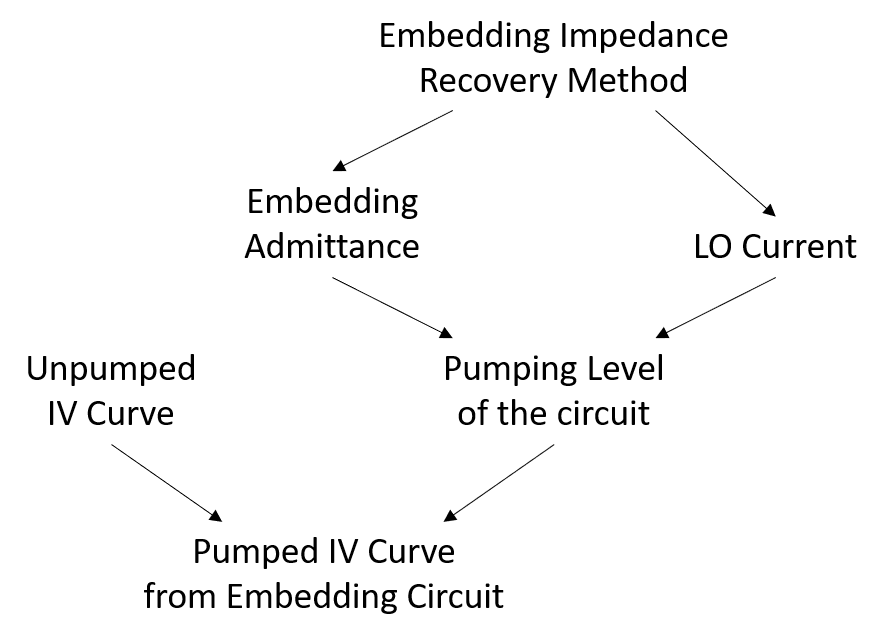
\includegraphics[width=0.7\textwidth]{./Images/Impedance_Recovery_Flowchart_Part2.png}
	\caption{The result of the embedding admittance can be used to reconstruct the pumped IV curve following this flowchart.}
	\label{fig:Result_Evaluation_Flowchart}
\end{figure}

\begin{figure}
	\centering
	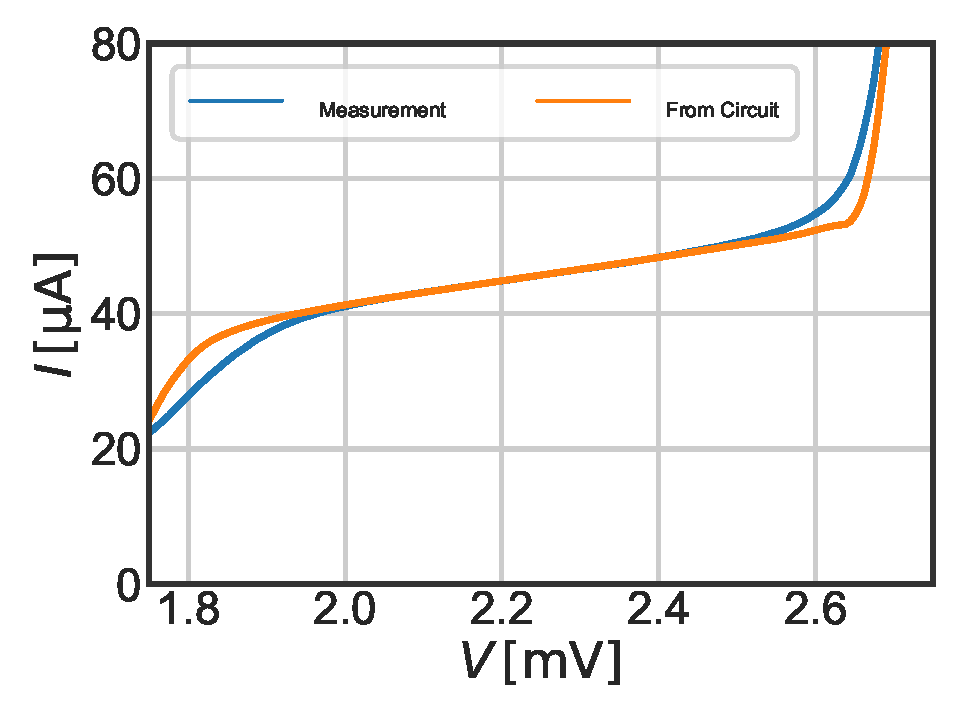
\includegraphics[width=0.7\textwidth]{../Mixer_Unit_Test/2020_01_12_GausMask/Pumped_Recovered.pdf}
	\caption{The pumped IV curve computed from the embedding impedance shows good agreement with the measured pumped IV curve over the voltage range of the first photon step. The embedding impedance recovery utilised the gaussian masking strategy.}
	\label{fig:Pumped_Recovered}
\end{figure}

\section{Results}
The presented software has been tested with example data from the QMix package to validate the results with the QMix results. Since the QMix package uses one photon step for the impedance recovery, the presented results are obtained from the first photon step unless otherwise stated.

The characteristics of the unpumped IV response obtained with the QMix package and the presented software are compared in table \ref{tab:IV}. The results agree in all parts except for the subgap resistance. This can be ascribed to the voltages from which the subgap resistance is obtained. QMix determines the subgap resistance at 2.0\,mV, while the presented software obtains the subgap resistance from a linear regression between 1.2\,mV and 1.8\,mV. The subgap resistance of the \texttt{IV\_Response} object results in 368.2\,\textOmega~by setting the limits for the linear regression to 1.9\,mV and 2.1\,mV. This agrees with the QMix result.

\begin{table}[]
	\centering
	\renewcommand{\arraystretch}{1.5}
	\begin{tabular}{l|c|c}
		 & Obtained Result & QMix Result \\\hline
		Gap Voltage [mV] & 2.71 & 2.72 \\
		Normal Resistance [\textOmega] & 13.68 & 13.41 \\
		Subgap Resistance [\textOmega] & 533.7 & 364.50 \\
		Voltage Offset [mV] & 0.10 & 0.10 \\
		Current Offet [\textmu A] & 9.62 & 9.67
	\end{tabular}
	\caption{The results of the unpumped IV curve are similar to the QMix results.}
	\label{tab:IV}
\end{table}

The QMix package's impedance recovery follows \cite{Withington1995} and results without modifications in $(6.30 - 4.02j)\,\Omega$ which corresponds with an embedding admittance of $(0.1128 + 0.0720j)\,\mho$. 
The QMix package evaluates the impedance at a defined set of resistances and reactances so that the result changes to $(6.45 - 4.21j)\,\Omega$ after increasing the number of evaluated resistances and reactances by a factor of 50 each.\footnote{The result requires changes in the \texttt{RawData} class of the QMix package under the path \texttt{qmix/exp/exp\_data.py}.} 
The pumped IV curve in figure \ref{fig:Comparison_with_Johns_Embedding_Impedance} is recovered from the QMix's embedding impedance result plugged into the \texttt{Mixer} class using pumping levels from the fixed voltage masking strategy with the same voltage limits as in the QMix package.
%The pumped IV curve recovered from the QMix result and the here presented script is shown in figure \ref{fig:Comparison_with_Johns_Embedding_Impedance} in comparison with the measured pumped IV curve. 
The plot also shows the result obtained with the presented software which is closer to the measured data.
%altering the grid into smaller steps of resistances and reactances so that about 50 times more points are evaluated.


\begin{figure}
	\centering
	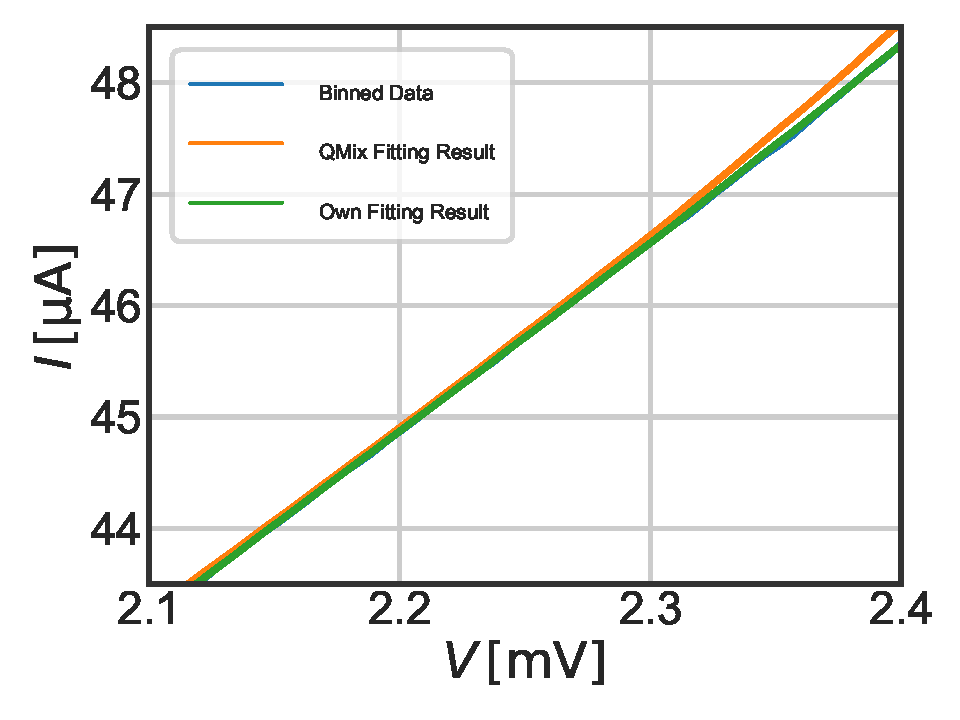
\includegraphics[width=0.7\textwidth]{../Mixer_Unit_Test/2020_01_14_GausMask/Comparison_with_Johns_Embedding_Impedance.pdf}
	\caption{The pumped IV curves computed from the QMix result and the here presented fitting methods agree well with the measured pumped IV response at the first photon step. The photon step is masked with the fixed voltage masking strategy and the limits used by the QMix package. Note that the blue Binned Data curve is mostly covered by the green line.}
	\label{fig:Comparison_with_Johns_Embedding_Impedance}
\end{figure}


The presented script uses two different masking strategies where the photon step extent is either reduced by four times the width of the gaussian fit on the transition or by a defined width. A comparison of the results for the masking strategies is shown in figure \ref{fig:Comparison_Masking_Strategy_Gaus_Fixed_Embedding_Impedance}. Furthermore, there is a difference between including data from only positive bias voltages, and including the data at photon steps with negative bias voltage. This is shown in figure \ref{fig:Comparison_Masking_Strategy_Embedding_Impedance}. The results for both masking strategies are presented in table \ref{tab:Yemb}. The results of the Skalare method, the Withington method, and the circuit evaluation method are consistent with the cost functions described in equations \ref{eq:cost_Skalare}, \ref{eq:cost_Withington} and \ref{eq:cost_own}, respectively. For example, where the eyeball method results in $(0.0669 + 0.0617j)\,\mho$ or $(8.08 - 7.45j)\,\Omega$ respectively, the other methods result in $(7.67 - 5.66j)\,\Omega$. This originates from the different approach for the eyeball method. However, the comparison of the resulting pumped IV curves in figure \ref{fig:Pumped_Recovered_Compaison} shows minor differences in the fitting region. There are two possibilities to explain the low difference between the results. Either the shape of the pumped IV curve is insensitive to the difference of the embedding admittance, or the evaluation of the pumped IV curve is chosen improperly. 
\begin{figure}
	\centering
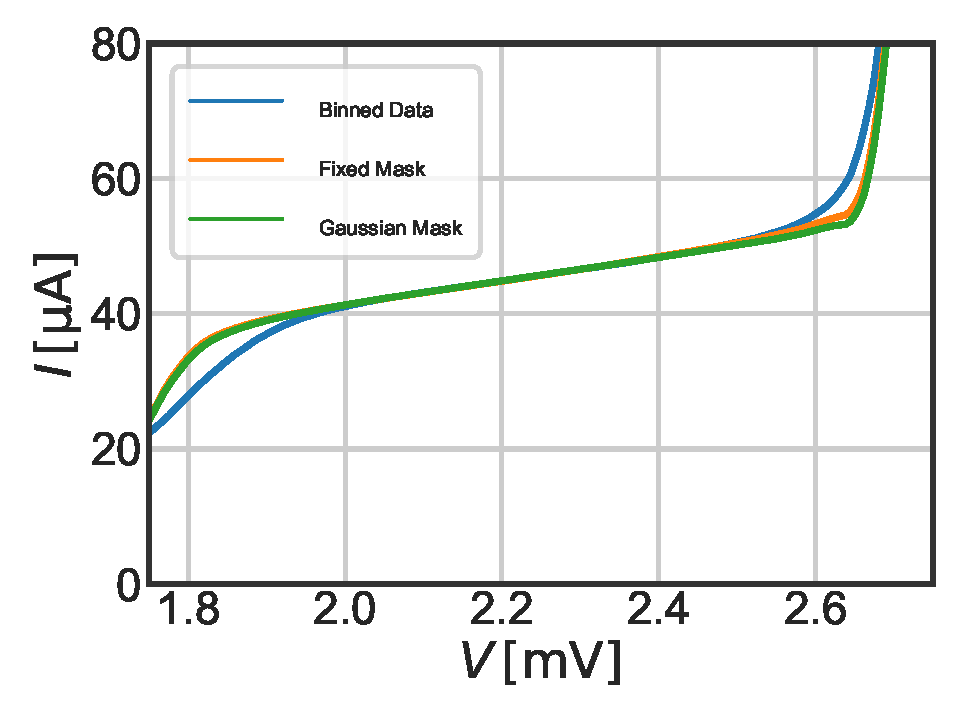
\includegraphics[width=0.7\textwidth]{../Mixer_Unit_Test/2020_01_14_Fixed_Mask/Comparison_Masking_Strategy_Gaus_Fixed_Embedding_Impedance.pdf}
\caption{The pumped IV curve computed from the fixed voltage masking strategy shows slightly better agreement close to the transition than the gaussian masking strategy. This can be ascribed to the fact that the fixed voltage masking strategy includes voltages beyond 2.5\,mV while the gaussian masking strategy includes voltages only up to 2.41\,mV.  }
\label{fig:Comparison_Masking_Strategy_Gaus_Fixed_Embedding_Impedance}
\end{figure}
\begin{figure}
	\centering
	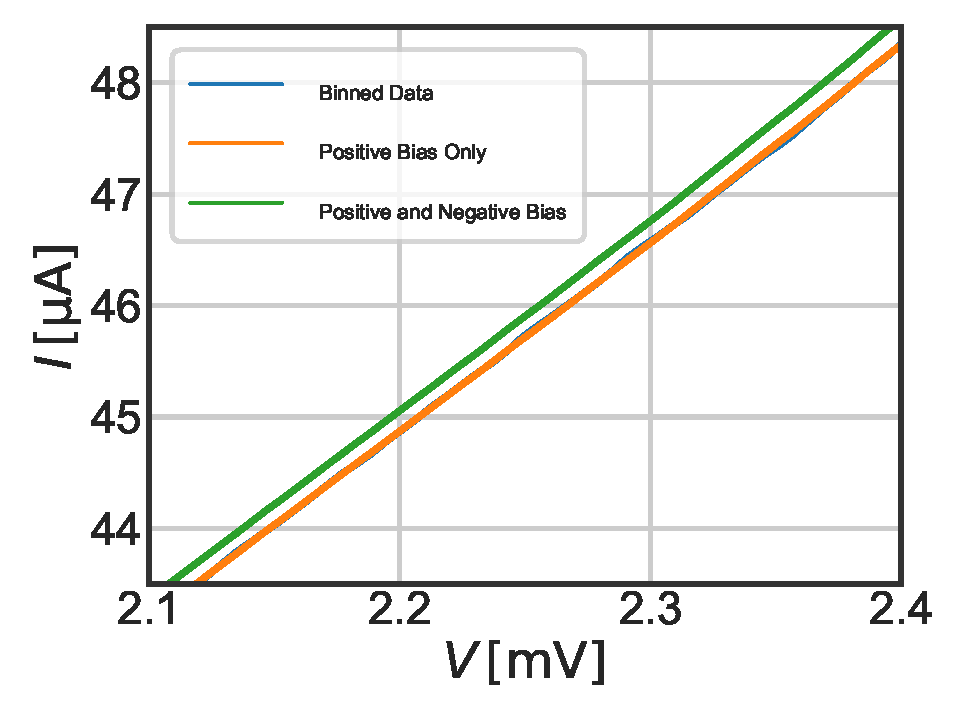
\includegraphics[width=0.7\textwidth]{../Mixer_Unit_Test/2020_01_14_GausMask/Comparison_Masking_Strategy_Voltage_Embedding_Impedance.pdf}
	\caption{The pumped IV curve computed from the masked photon step at positive bias voltages shows good agreement with the binned IV curve in the positive voltage range. The recovered binned IV curve from results obtained in negative and positive bias voltage regions is offset, since the pumping level at negative bias voltages is of slightly larger magnitude. }
	\label{fig:Comparison_Masking_Strategy_Embedding_Impedance}
\end{figure}

\begin{table}[]
	\centering
	\renewcommand{\arraystretch}{1.5}
	\begin{tabular}{l|cc|cc}
		\hline
		Pos. and Neg. & \multicolumn{2}{c|}{Gaussian Masking Limits} & \multicolumn{2}{c}{Defined Masking Limits} \\
		Voltages& $Y_\text{emb}$ [$\mho$] & $I_\text{LO}$ [\textmu A] & $Y_\text{emb}$ [$\mho$] & $I_\text{LO}$ [\textmu A] \\\hline
		Skalare & 0.0844 + 0.0623j & 166.8 & 0.1033 + 0.0703j & 184.7 \\
		Cost Function & 0.0844 + 0.0623j & 166.2 & 0.1033 + 0.0703j & 184.7 \\
		Eyeball & 0.0669 + 0.0617j & 152.0 & 0.1311 + 0.0771j & 209.4 \\
		Withington & 0.0844 + 0.0623j &  & 0.1033 + 0.0703j &  \\
		\hline
		Positive Voltages & \multicolumn{2}{c|}{Gaussian Masking Limits} & \multicolumn{2}{c}{Defined Masking Limits} \\
		& $Y_\text{emb}$ [$\mho$] & $I_\text{LO}$ [\textmu A] & $Y_\text{emb}$ [$\mho$] & $I_\text{LO}$ [\textmu A] \\\hline
		Skalare & 0.0793 + 0.0604j & 161.5 & 0.0950 + 0.0675j & 176.5 \\
		Cost Function & 0.0793 + 0.0604j & 161.5 & 0.0950 + 0.0675j & 176.5 \\
		Eyeball & 0.0687 + 0.0572j & 151.8 & 0.0940 + 0.0665j & 175.4 \\
		Withington & 0.0793 + 0.0604j &  & 0.0950 + 0.0675j & 
	\end{tabular}
	\caption{The results of the different evaluation methods are listed for both masking strategies, where in the upper panel positive and negative bias voltages are used, and only positive bias voltages are evaluated in the lower panel results.}
	\label{tab:Yemb}
\end{table}
\begin{figure}
\centering
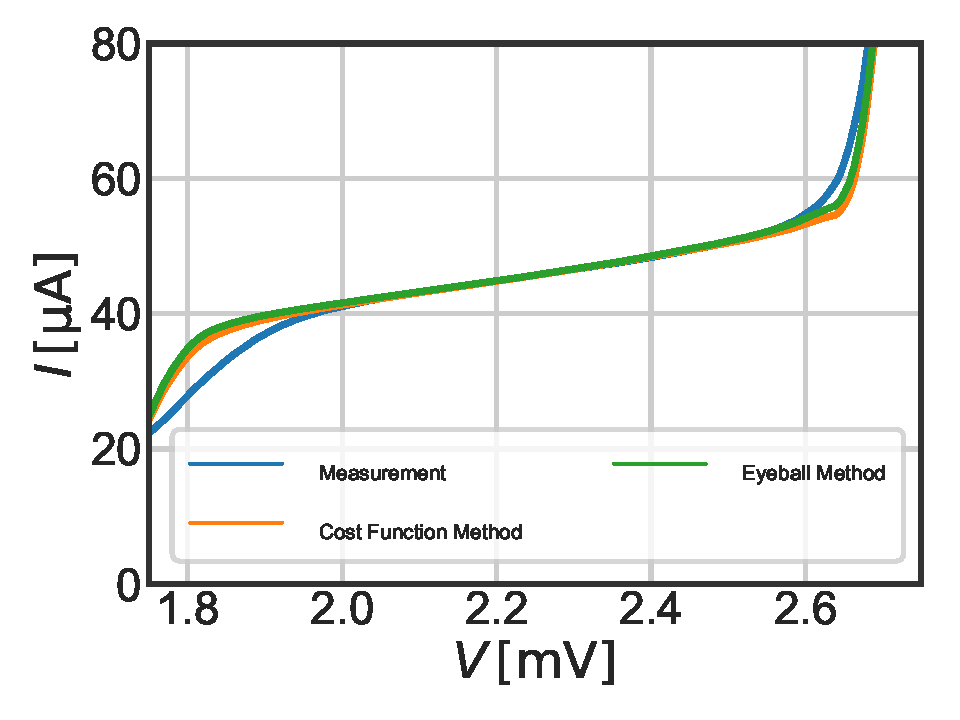
\includegraphics[width=0.7\textwidth]{../Mixer_Unit_Test/2020_01_14_Fixed_Mask/Pumped_Recovered_Comparison.pdf}
\caption{The pumped IV curves computed with the cost function methods and the eyeball method show similar results and good agreement with the measured IV curve.}
\label{fig:Pumped_Recovered_Compaison}
\end{figure}

Finally, there is the possibility to use the second photon step in addition to the first photon step as shown in figure \ref{fig:Masked_Voltage_Region_two_Photon_Steps}. In general, the second photon step is considered too noisy to perform the embedding admittance recovery on this data. Figure \ref{fig:Pumping_Level}, however, shows a well defined pumping level in the region of the second photon step. The results for the embedding admittance obtained with both masking strategies over two photon steps are presented in table \ref{tab:yEmb2Steps}. Figure \ref{fig:Pumped_Recovered_Comparison_Two_Photon_Steps} shows good agreement between the measurement and the recovered pumped IV curve. Interestingly, the result, which includes the data at bias voltages between the first and second photon step, shows good agreement at the photon steps themselves and shows better agreement at the voltages between the photon steps. In conclusion, the results obtained by including two photon steps show better agreement with the pumped IV curve than the results obtained from one photon step.
%TODO add a table with the results of two photon steps continuous

\begin{figure}
	\centering              
	\begin{subfigure}[t]{0.49\textwidth}
		\centering
		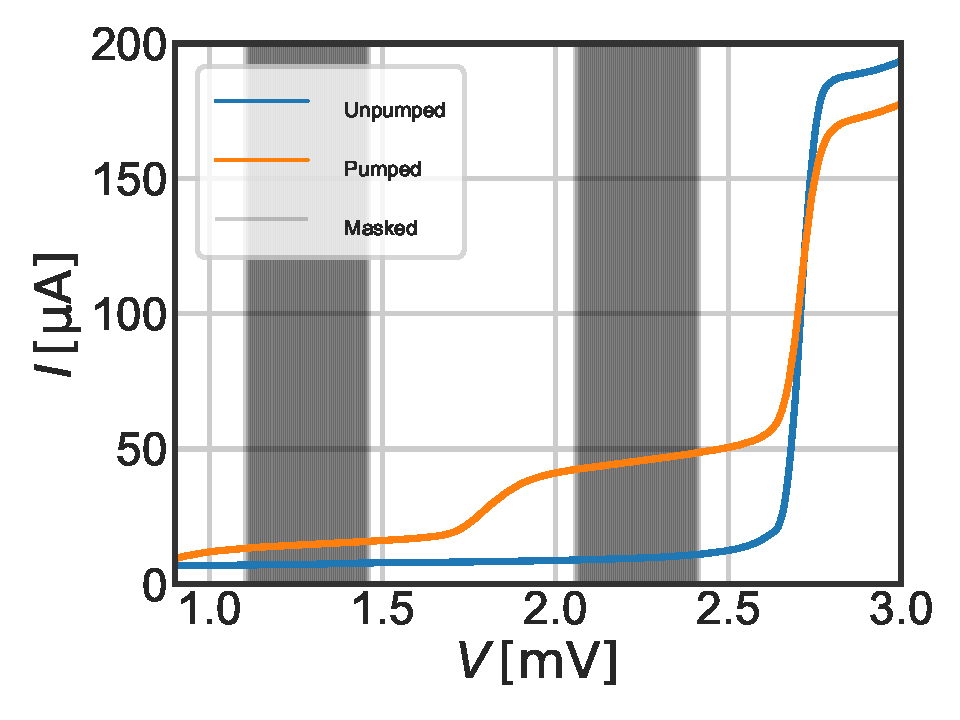
\includegraphics[width=\linewidth]{./../Mixer_Unit_Test/2020_01_15_Gaus_Two_Steps/Masked_Voltage_Region_two_Photon_Steps.pdf}
		\caption{The evaluated bias voltage region originates from the gaussian masking strategy.}
	\end{subfigure}
	\begin{subfigure}[t]{0.49\textwidth}
		\centering
		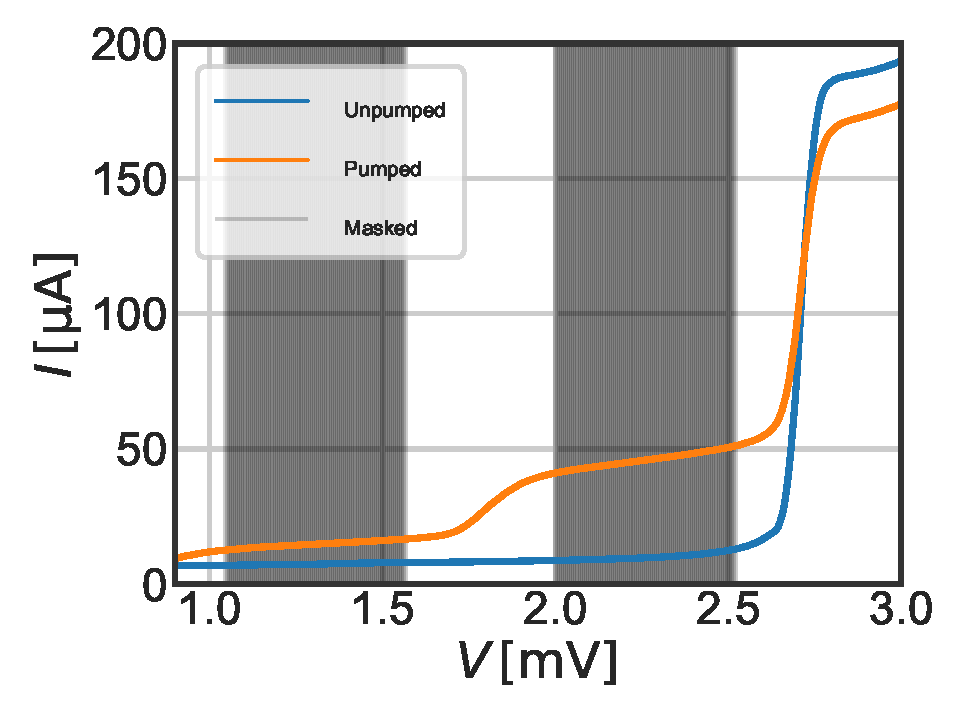
\includegraphics[width=\linewidth]{./../Mixer_Unit_Test/2020_01_15_twoPhotonStepsFixed/Masked_Voltage_Region_two_Photon_Steps.pdf}
		\caption{The evaluated bias voltage region originates from the fixed voltage masking strategy.}
	\end{subfigure}
	\caption[]{The bias voltage selection strategies for the impedance recovery are shown for the first two photon steps.
	}
	\label{fig:Masked_Voltage_Region_two_Photon_Steps}
\end{figure}

\begin{table}[]
	\centering
	\renewcommand{\arraystretch}{1.5}
	\begin{tabular}{l|cc|cc}\hline
		Pos. and Neg. & \multicolumn{2}{c|}{Gaussian Masking Limits} & \multicolumn{2}{c}{Defined Masking Limits} \\
		Voltages & $Y_\text{emb}$ [$\mho$] & $I_\text{LO}$ [\textmu A] & $Y_\text{emb}$ [$\mho$] & $I_\text{LO}$ [\textmu A] \\\hline
		Skalare & 0.0702 + 0.0586j & 153.9 & 0.0705 + 0.0586j & 154.4 \\
		Cost Function & 0.0702 + 0.0586j & 153.9 & 0.0702 + 0.0586j & 153.9 \\
		Eyeball & 0.1744 + 0.0857j & -0.01 & 0.1736 + 0.0863j & 0.003 \\
		Withington & 0.0702 + 0.0586j &  & 0.0702 + 0.0586j &  \\\hline
		Positive Voltages & \multicolumn{2}{c|}{Gaussian Masking Limits} & \multicolumn{2}{c}{Defined Masking Limits} \\
		& $Y_\text{emb}$ [$\mho$] & $I_\text{LO}$ [\textmu A] & $Y_\text{emb}$ [$\mho$] & $I_\text{LO}$ [\textmu A] \\\hline
		Skalare & 0.0697 + 0.0583j & 153.0 & 0.0698 + 0.0584j & 153.3 \\
		Cost Function & 0.0697 + 0.0583j & 153.0 & 0.0698 + 0.0584j & 153.3 \\
		Eyeball & 0.0714 + 0.0579 & 154.3 & 0.0664 + 0.0587 & 150.3 \\
		Withington & 0.0697 + 0.0583j &  & 0.0698 + 0.0584j & 
	\end{tabular}
	\caption{The results for the embedding admittance by using data from the first and second photon step show good results, except for the Eyeball method applied on negative and positive bias voltages.}
	\label{tab:yEmb2Steps}
\end{table}

\begin{figure}
	\centering              
	\begin{subfigure}[t]{0.49\textwidth}
		\centering
		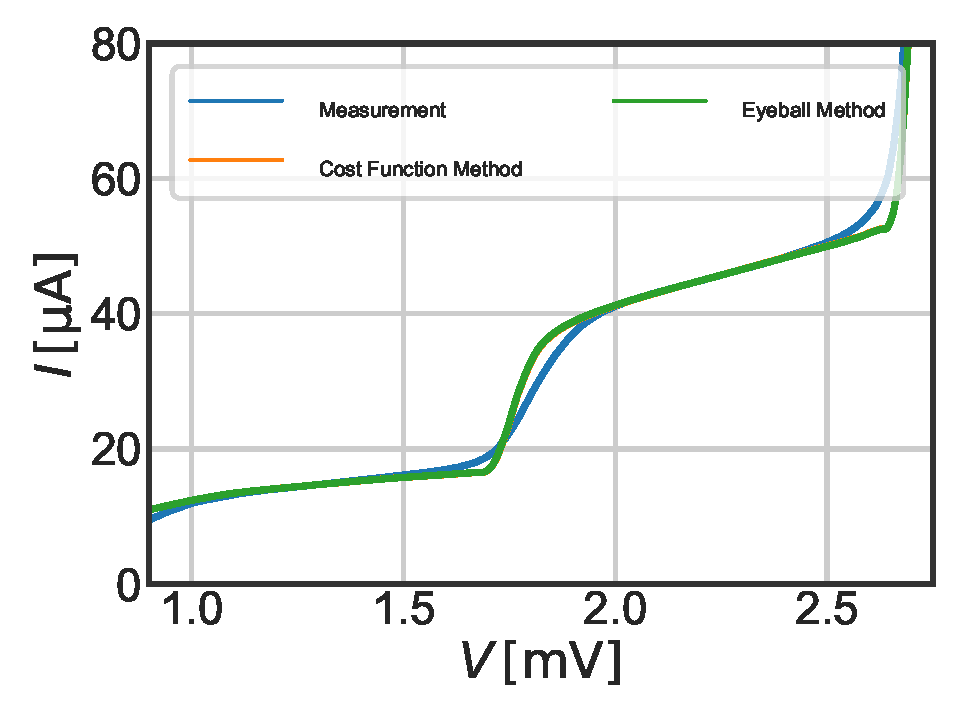
\includegraphics[width=\linewidth]{./../Mixer_Unit_Test/2020_01_15_Gaus_Two_Steps/Pumped_Recovered_Comparison_Two_Photon_Steps.pdf}
		\caption{The gaussian masking strategy on two photon steps.}
	\end{subfigure}
	\begin{subfigure}[t]{0.49\textwidth}
		\centering
		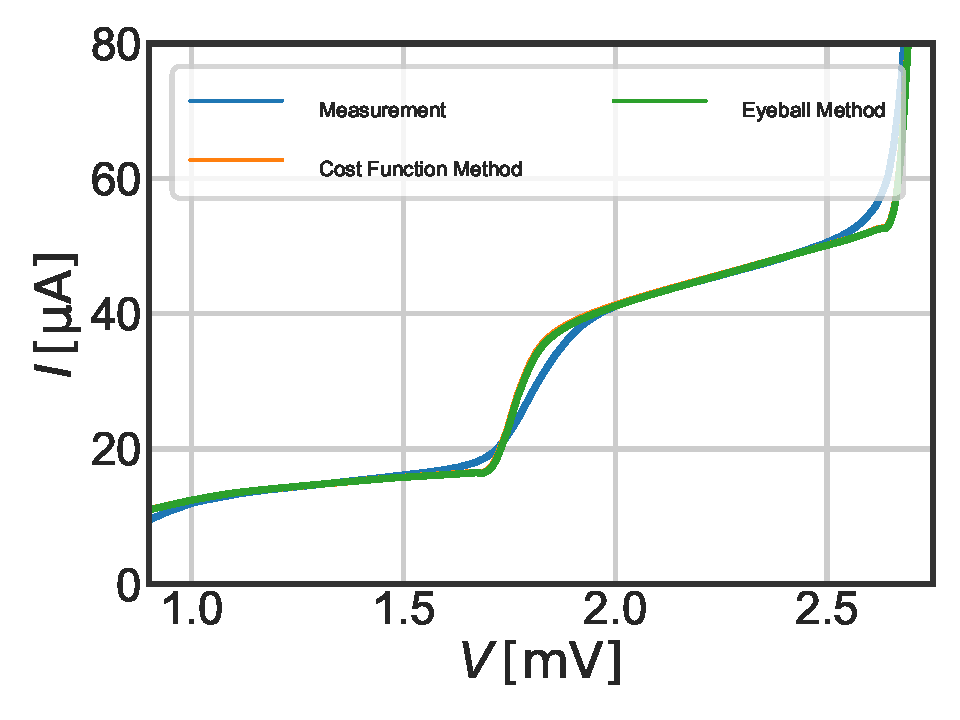
\includegraphics[width=\linewidth]{./../Mixer_Unit_Test/2020_01_15_twoPhotonStepsFixed/Pumped_Recovered_Comparison_Two_Photon_Steps.pdf}
		\caption{The fixed voltage range masking strategy on two photon steps.}
	\end{subfigure}
\begin{subfigure}[t]{0.49\textwidth}
	\centering
	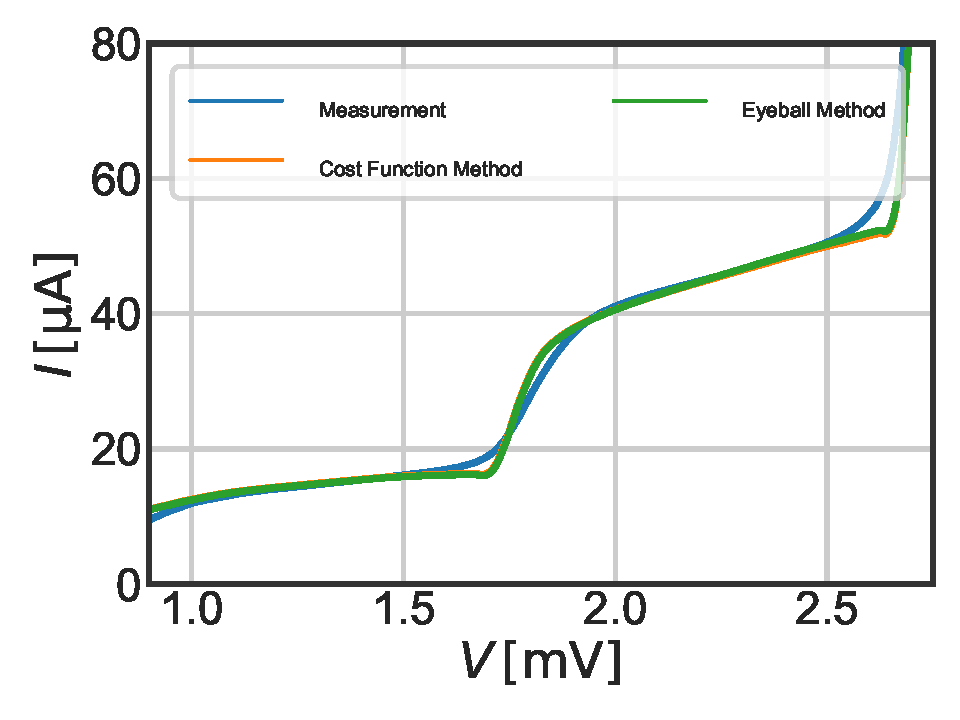
\includegraphics[width=\linewidth]{./../Mixer_Unit_Test/2020_01_15_FixedMask_Continuous_Over_Two_Photonsteps/Pumped_Recovered_Comparison_Two_Photon_Steps.pdf}
	\caption{This result is obtained from the extended voltage range of the fixed voltage range masking strategy, which includes the bias voltages between the first and second photon step.}
\end{subfigure}
\begin{subfigure}[t]{0.49\textwidth}
	\centering
	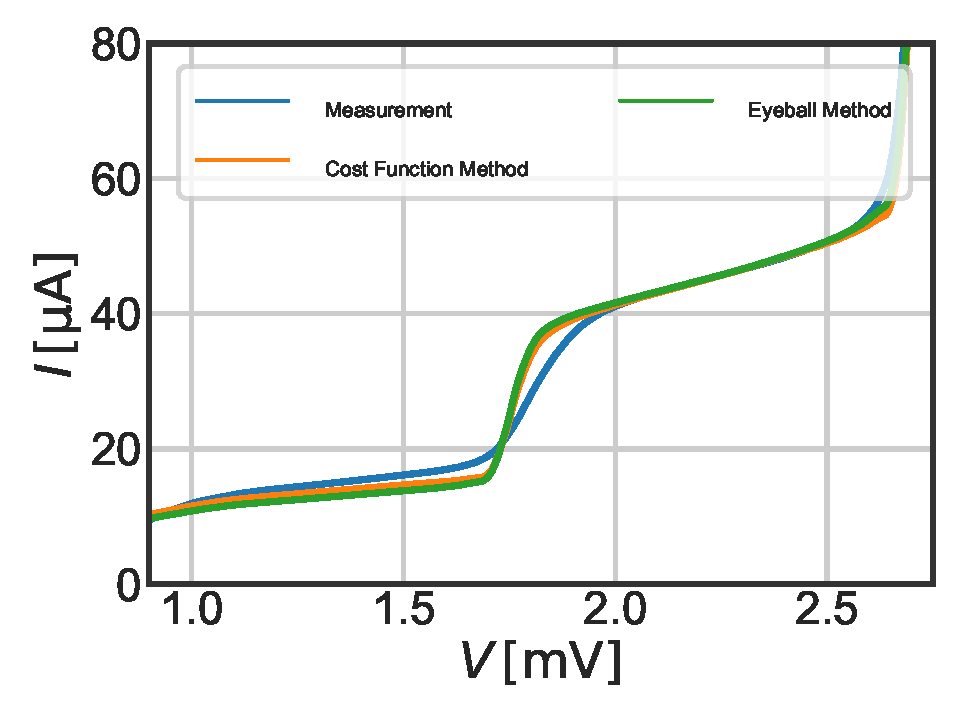
\includegraphics[width=\linewidth]{./../Mixer_Unit_Test/2020_01_14_Fixed_Mask/Pumped_Recovered_Comparison_Two_Photon_Steps.pdf}
	\caption{This result is obtained from the first photon step only and the fixed voltage masking strategy.}
\end{subfigure}
	\caption[]{This figure compares the results obtained with different masking strategies applied on two photon steps (a-c) and one photon step (d). The results obtained in (a) and (b) are very similar, but both Eyeball evaluations fail as negative bias voltages are included in the evaluation.
	}
	\label{fig:Pumped_Recovered_Comparison_Two_Photon_Steps}
\end{figure}

\section{Discussion}
In this final discussion section, the impact of the IV curve offset is discussed with respect to the discrepancy of our results to the QMix result. Figure \ref{fig:OffsetIVcurve} shows the origin of the measured IV curves with different offset settings and in figure \ref{fig:Offseted_PumpedIVcurve}, the corresponding recovered pumped IV curves are compared. The embedding admittances and impedances with respect to the photon step masking strategy and the used offset are listed in table \ref{tab:OffsetedData}. Note that the user define offset is applied on the unpumped IV curve only, and that the offset correction of the pumped IV curve is computed automatically in the \texttt{IV\_Response} object following the description earlier. The voltage offset 0.101802\,mV is determined by the \texttt{IV\_Response} object on the unpumped IV curve. The offset has been partially chosen in a way to overlap the pumping level of the first photon step at negative and positive bias voltage regions as shown in figure \ref{fig:OffsetedPumpingLevels}.

\begin{figure}
	\centering              
	\begin{subfigure}[t]{0.49\textwidth}
		\centering
		\includegraphics[width=\linewidth]{./../Mixer_Unit_Test/2020_01_16_IVOffsetFixedMask_9.8uA/Unpumped_Pumped_Offset_Zoom.pdf}
		\caption{A set current offset of 9.8 \textmu A.}
	\end{subfigure}
	\begin{subfigure}[t]{0.49\textwidth}
		\centering
		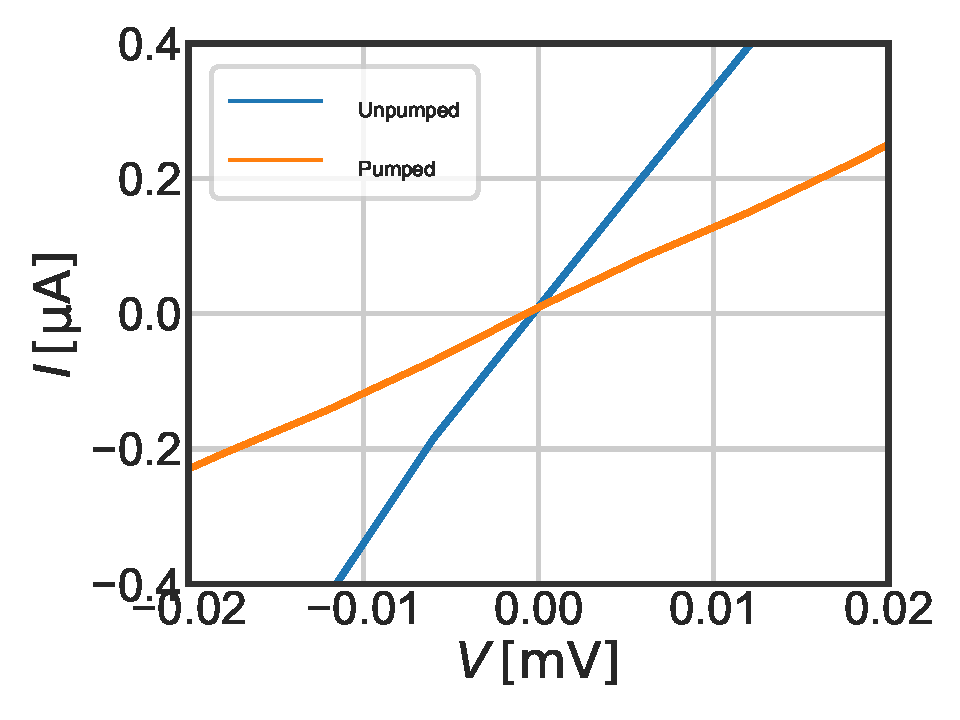
\includegraphics[width=\linewidth]{./../Mixer_Unit_Test/2020_01_16_IVOffsetFixedMask_0.105mV9.8uA/Unpumped_Pumped_Offset_Zoom.pdf}
		\caption{A set voltage offset of 0.105\,mV and a set current offset of 9.8 \textmu A.}
	\end{subfigure}
	\begin{subfigure}[t]{0.49\textwidth}
		\centering
		\includegraphics[width=\linewidth]{./../Mixer_Unit_Test/2020_01_16_IVOffsetGausMask_9.8uA/Unpumped_Pumped_Offset_Zoom.pdf}
		\caption{A set current offset of 9.8 \textmu A.}
	\end{subfigure}
	\begin{subfigure}[t]{0.49\textwidth}
		\centering
		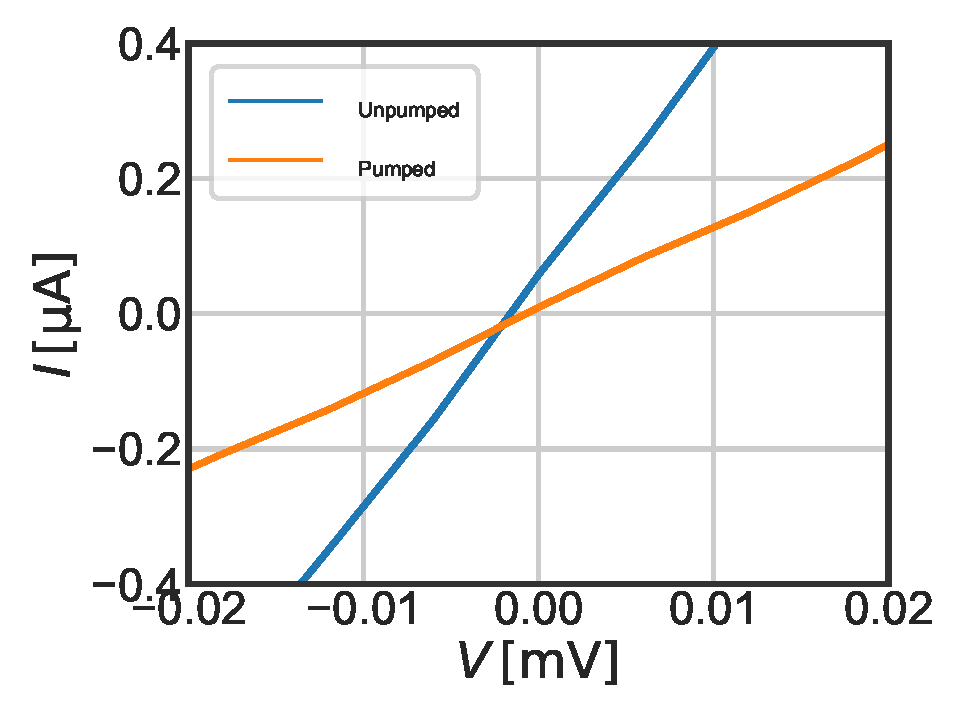
\includegraphics[width=\linewidth]{./../Mixer_Unit_Test/2020_01_14_Fixed_Mask_iLOfix/Unpumped_Pumped_Offset_Zoom.pdf}
		\caption{The automatic offset correction by the \texttt{IV\_Response} class. }
	\end{subfigure}
	\caption[]{This figure shows the offset of the unpumped and pumped IV curve close to the origin. The order corresponds with the order of table \ref{tab:OffsetedData}.
	}
	\label{fig:OffsetIVcurve}
\end{figure}

\begin{figure}
	\centering              
	\begin{subfigure}[t]{0.49\textwidth}
		\centering
		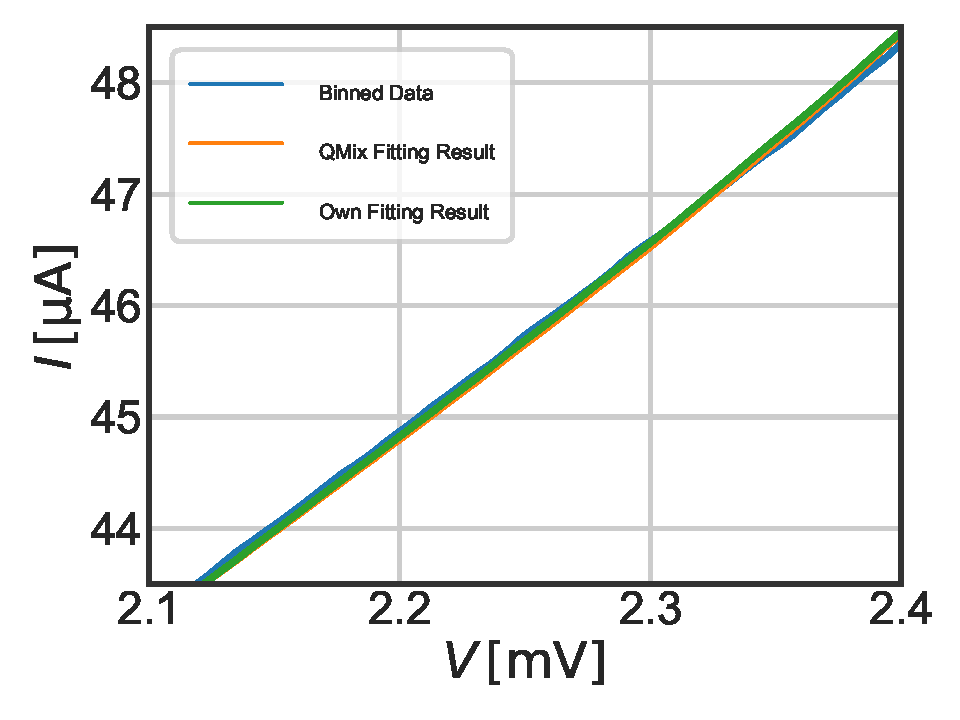
\includegraphics[width=\linewidth]{./../Mixer_Unit_Test/2020_01_16_IVOffsetFixedMask_9.8uA/Comparison_with_Johns_Embedding_Impedance.pdf}
		\caption{A set current offset of 9.8 \textmu A evaluated with the fixed masking strategy.}
	\end{subfigure}
	\begin{subfigure}[t]{0.49\textwidth}
		\centering
		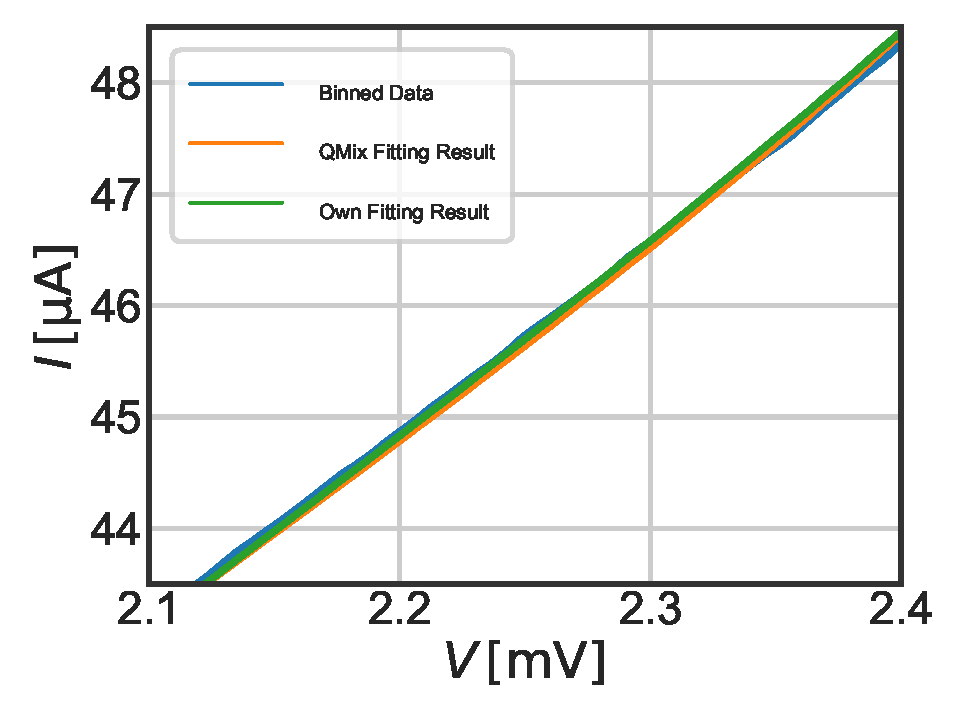
\includegraphics[width=\linewidth]{./../Mixer_Unit_Test/2020_01_16_IVOffsetFixedMask_0.105mV9.8uA/Comparison_with_Johns_Embedding_Impedance.pdf}
		\caption{A set voltage offset of 0.105\,mV and current offset of 9.8 \textmu A evaluated with the fixed masking strategy.}
	\end{subfigure}
	\begin{subfigure}[t]{0.49\textwidth}
		\centering
		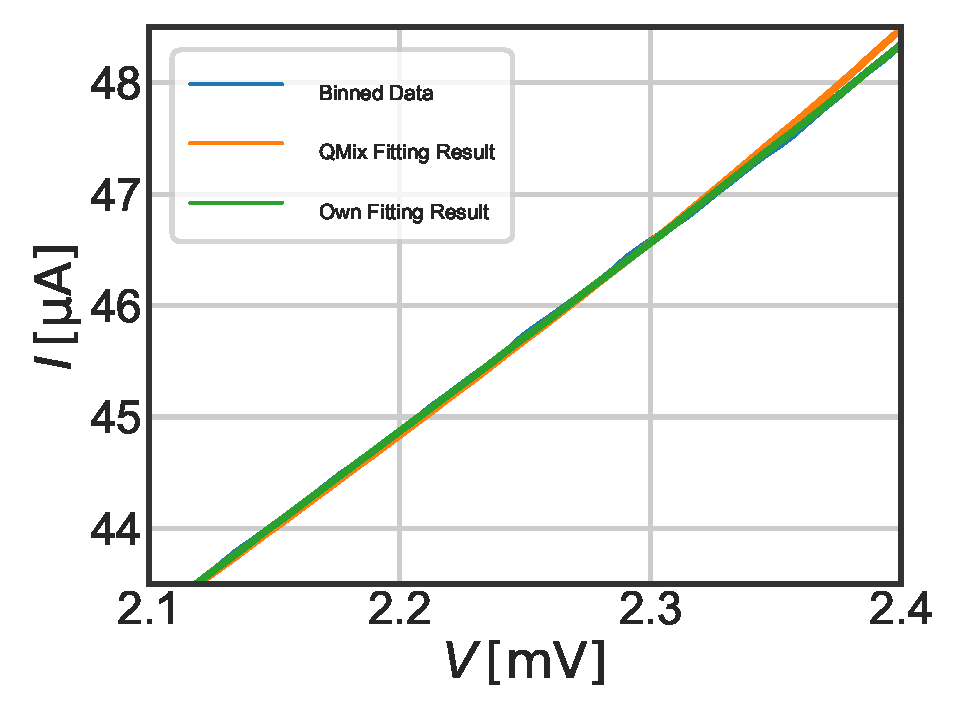
\includegraphics[width=\linewidth]{./../Mixer_Unit_Test/2020_01_14_IVOffset_9.8uA_iLOfix/Comparison_with_Johns_Embedding_Impedance.pdf}
		\caption{A set current offset of 9.8 \textmu A evaluated with the gaussian masking strategy.}
	\end{subfigure}
	\begin{subfigure}[t]{0.49\textwidth}
		\centering
		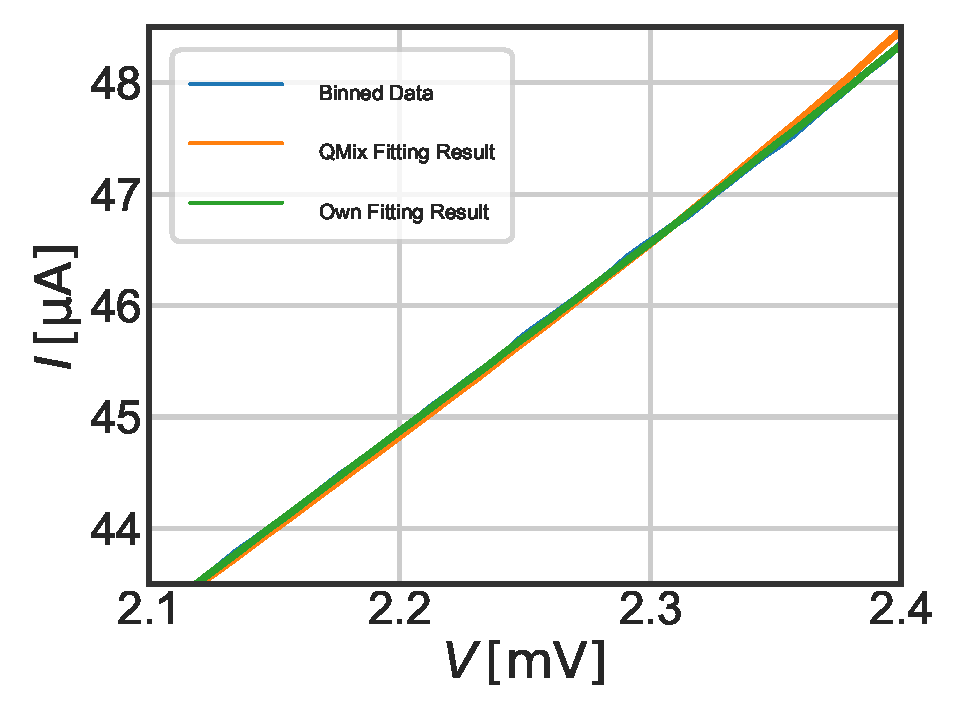
\includegraphics[width=\linewidth]{./../Mixer_Unit_Test/2020_01_16_IVOffsetGausMask_9.8uA/Comparison_with_Johns_Embedding_Impedance.pdf}
		\caption{The automatic result with fixed masking strategy.}
	\end{subfigure}
	\caption[]{A comparison of the pumped IV curve recovered from the embedding admittance is shown for different IV curve offset settings at the first photon step. The QMix result varies, since during the recovery of the pumped IV curve the $I_\text{LO}$ is computed from the masked pumping levels. A different masking strategy and a different voltage offset has impact on the $I_\text{LO}$. Note that the order corresponds with the order of table \ref{tab:OffsetedData}.
	}
	\label{fig:Offseted_PumpedIVcurve}
\end{figure}
\begin{table}[]
	\centering
	\renewcommand{\arraystretch}{1.5}
	\begin{tabular}{ccccc}\hline
		$V_\text{offset}$ & $I_\text{offset}$ & Masking & $Y_\text{emb}$ [$\mho$]  & $Y_\text{emb}$ [$\mho$]\\
		&&Strategy&Pos. \& Neg. Bias&Pos. Bias \\\hline
		0.101802 & 9.8 & Fixed & 0.1045+0.0705j & 0.0955+0.0673j \\
		0.105 & 9.8 & Fixed & 0.0949 + 0.0677j & 0.0870 +0.0650j \\
		0.101802 & 9.8 & Gaus & 0.0874 + 0.0631j & 0.0797 + 0.0604 \\
		automatic & automatic & Fixed & 0.1033 + 0.0703j & 0.0950 + 0.0675j \\\hline
		$V_\text{offset}$ & $I_\text{offset}$ & Masking  & $Z_\text{emb}$ [$\Omega$] & $Z_\text{emb}$ [$\Omega$] \\
		&&Strategy&Pos. \& Neg. Bias&Pos. Bias \\\hline
		0.101802 & 9.8 & Fixed & 6.58-4.44j & 6.99-4.93j \\
		0.105 & 9.8 & Fixed & 6.98 - 4.98j & 7.37 - 5.51j \\
		0.101802 & 9.8 & Gaus & 7.52 - 5.43j & 7.98 - 6.04j \\
		automatic & automatic & Fixed & 6.61 - 4.50j & 6.99-4.97j
	\end{tabular}
\caption{The upper panel shows the embedding admittance results and the lower panel shows the embedding impedance results for different offset settings. The first entry in both panels has similar results as the QMix package and uses the same masking strategy as the QMix package. With respect to this, an additional voltage offset with the same masking strategy is evaluated, a result with gaussian masking strategy with the same offset as the first entry is evaluated, and finally an entry with the automatically calculated offset is given as comparison. }
\label{tab:OffsetedData}
\end{table}
\begin{figure}
	\centering              
	\begin{subfigure}[t]{0.49\textwidth}
		\centering
		\includegraphics[width=\linewidth]{./../Mixer_Unit_Test/2020_01_16_IVOffsetFixedMask_9.8uA/Pumping_Level_Zoom.pdf}
		\caption{A set current offset of 9.8 \textmu A.}
	\end{subfigure}
	\begin{subfigure}[t]{0.49\textwidth}
		\centering
		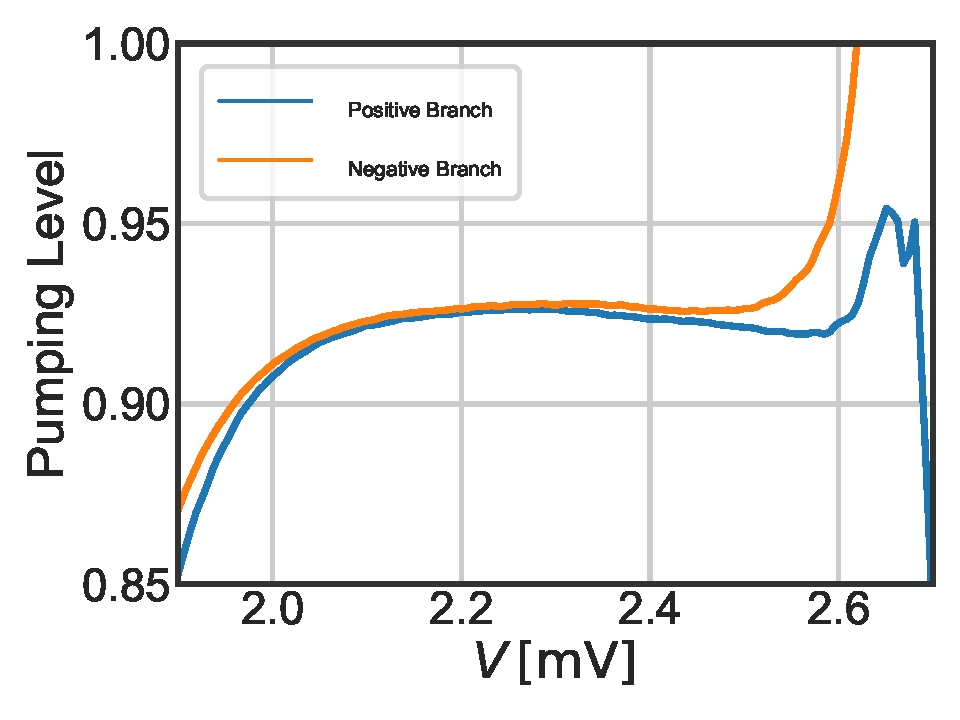
\includegraphics[width=\linewidth]{./../Mixer_Unit_Test/2020_01_16_IVOffsetFixedMask_0.105mV9.8uA/Pumping_Level_Zoom.pdf}
		\caption{A set voltage offset of 0.105\,mV and a set current offset of 9.8 \textmu A.}
	\end{subfigure}
	\begin{subfigure}[t]{0.49\textwidth}
		\centering
		\includegraphics[width=\linewidth]{./../Mixer_Unit_Test/2020_01_16_IVOffsetGausMask_9.8uA/Pumping_Level_Zoom.pdf}
		\caption{A set current offset of 9.8 \textmu A.}
	\end{subfigure}
	\begin{subfigure}[t]{0.49\textwidth}
		\centering
		\includegraphics[width=\linewidth]{./../Mixer_Unit_Test/2020_01_14_Fixed_Mask_iLOfix/Pumping_Level_Zoom.pdf}
		\caption{The automatic offset correction by the \texttt{IV\_Response} class. }
	\end{subfigure}
	\caption[]{The pumping level recovered from the unpumped and pumped IV curve are matched as a offset is introduced. Note that the order corresponds with the order of table \ref{tab:OffsetedData}.
	}
	\label{fig:OffsetedPumpingLevels}
\end{figure}

The recovery of the pumped IV curve from the QMix embedding impedance result entails problems with the calculation of the $I_\text{LO}$ following equation \ref{eq:ILO_Skalare}, since the equation contains the pumping level $V_\text{LO}(V_0)$. The bias voltages used by the \texttt{Mixer} object at which the pumping level is determined must not be necessarily exactly the same as in the QMix package, even the fixed voltage masking strategy is used with the same limits as in the QMix package. A difference in the gap voltage give raise to an offset in the determined bias voltage range. For this reason, the recovered pumped IV curve from the QMix embedding impedance result vary with the offset on the IV curve data as well as with the used masking strategy for the photon step. This can be seen for instance in figure \ref{fig:Offseted_PumpedIVcurve}.

The four entries in figure \ref{fig:OffsetIVcurve}, \ref{fig:Offseted_PumpedIVcurve} and \ref{fig:OffsetedPumpingLevels} and table \ref{tab:OffsetedData} correspond in their order. The first entry is chosen to achieve a result for the embedding impedance close to the QMix result. As can be seen in figure \ref{fig:OffsetIVcurve}, this result is not obtained at a perfect offset correction. The second entry introduced an additional voltage offset of about 0.003\,mV to set the measured unpumped IV curve back to the origin. This, however, increases the result for the embedding impedance by $(0.40-0.44j)\,\Omega$. The third entry used the gaussian masking strategy on the offset settings of the first entry, and results in a larger magnitude for the embedding impedance. The last entry used the offset obtained from the \texttt{IV\_Response} object of the unpumped IV curve. The difference in offset are additional 0.18\,\textmu A, which correspond with a difference of less than $(0.10-0.10j)\,\Omega$ in the embedding impedance results. In general, the result by evaluating only positive bias voltages results in larger embedding impedances.

The results of different masking strategies and evaluated voltages, applied on the first photon step in table \ref{tab:Yemb}, on two photon steps in table \ref{tab:yEmb2Steps} and by introducing an offset in table \ref{tab:OffsetedData}, suggest that the impedance recovery can be seen as a rough guess value with a relative large error in the 10\% regime. However, the recovered pumped IV curves show good agreement with the measured pumped IV curve in all cases.
It is obvious that the IV curve offset has a strong impact on the pumping level and the following impedance recovery as shown in figure \ref{fig:OffsetedPumpingLevels}. In the same way, the impedance recovery result depends strongly on the bias voltage range in which the impedance recovery is performed. In general, the larger the bias voltage range, the smaller is the sensitivity of the recovery on noise. This noise can not only be introduced by the measurement, but also by physical backgrounds. An example is the Shapiro steps, which is negligible in the presented IV curves. Inclusion of data from the second photon step increases the bias voltage range used in the evaluation significantly. This, however, is not supported by literature and general practise. The inclusion of the photon steps at negative bias voltages is helpful in a way that the offset in the IV curve is accounted for. Nonetheless, this does not substitute the IV curve offset correction, since the pumping level recovery does not propagate the error linearly.

\section{Conclusion}
The presented software is able to determine the characteristic values of an IV response and the RF characteristics of a mixer. The used methods are described with references to the developed Python script. Testing and validation is obtained in conjunction with the QMix package. The results for the IV response agree with the exception of the subgap resistance, which can be ascribed to the different bias voltages evaluated. The obtained results for the embedding admittance agree with the measured data after recovering a pumped IV curve from the embedding admittance result in all cases. This leads to the conclusion that the recovered admittance is associated with large errors in the 10\% regime. The strategies of selecting the bias voltage range on which the recovery is performed has certainly an impact on the result. In the same way, the result varies as photon steps only from positive bias voltages are considered or if also negative bias voltages are included in the computation. The inclusion of the second photon step leads to better agreement of the result with the measured pumped IV curve in the second photon step, while the result still agrees within the first photon step. Finally, the impact of the offset correction has been briefly discussed, which has an impact on the obtained result for the embedding admittance.

\bibliographystyle{abbrvnat}
\bibliography{bibfile}

\end{document}
%
%
%
%OLD STUFF from here
%\section{Introduction} 
%
%Motivation of this work
%
%Why is it necessary to know how the Mixer characteristics
%-->the designing becomes clearer
%
%From what do I know the Mixer characteristics
%IV curves, IF curves
%
%\section{IV Curve Class}
%
%The SIS structure leads to a typical direct current (DC) voltage (IV) response. Experimentally, this response is obtained by sweeping the voltage up and down to conserve hysteresis behaviour. The voltage sweeping limits, the number of data points and a few other parameters depending on the experimental setup are controlled with a Labview readout programm. The program stores the data in `.csv` files with the following format, where the program has no header.
%
% Timestamp  Voltage [mV]  Current[$\mu$A]  
%
%\begin{table}
%	\centering
%	\caption{TableName}
%	\begin{tabular}{|l|l|l|}
%		\hline
%		
%		25/10/2019  15:34:49.011270 & 2.402918E0 & 1.319225E2 \\ \hline
%		25/10/2019  15:34:49.011436 & 2.413401E0 & 1.321199E2 \\ \hline
%		25/10/2019  15:34:49.011603 & 2.406849E1 & 1.322514E3 \\ \hline
%		25/10/2019  15:34:49.011770 & 2.408815E2 & 1.303439E4 \\ \hline
%		
%	\end{tabular}
%\end{table}
%
%The developed \texttt{IV\_Reponse()} class is designed to read IV curve tables and to compute the IV curves characteristics. The format of the input file can be defined through keyword arguments `**kwargs`, specifically
%- `headerLines`' defines how many lines from the top of the raw data file are skipted.
%- `footerLines` defines how many lines at the bottom of the raw data file are skipted. It is necessary to be defined if the file contains empty lines at its end.
%- `columnOffset` defines how many columns need to be skipped to get to the voltage column.
%
%In consequence, the \texttt{IV\_Reponse()} class is not unconfined to the format as long as there is a voltage data column left next to a current data column. 
%
%The presented testing uses data from QMix examples, which are in the format 
%\begin{table}
%	\centering
%	\caption{TableName}
%	\begin{tabular}{|l|l|}
%		\hline
%		
%		DC Bias Voltage (mV) & DC Tunneling Current (mA) \\ \hline
%		0.016102 & 0.007249 \\ \hline
%		0.017391 & 0.007265 \\ \hline
%		0.019324 & 0.007361 \\ \hline
%		0.021257 & 0.007378 \\ \hline
%		0.023512 & 0.007426 \\ \hline
%		0.026090 & 0.007474 \\ \hline
%		
%	\end{tabular}
%\end{table}
%where the file also contains the header line. 
%
%The dataset contains a sweep up and down in voltage which is stored as argument `rawIVData`.
%
%\begin{figure}
%	\centering
%	%\includegraphics[width=0.5\textwidth]{./IV_Class_Unit_Test/2020_01_02/Raw_Data_by_Time.pdf}
%	\caption{}
%\end{figure}
%
%
%
%The raw data is used to determine the offset. At the 0 V bias voltage and 0 A current, the slope in the subgap region shows a maximum. This can be seen from a plot of the `rawIVData`. 
%
%\begin{figure}
%	\centering
%	%\includegraphics[width=0.5\textwidth]{./IV_Class_Unit_Test/2020_01_02/Raw_Data_at_Origin.pdf}
%	\caption{}
%\end{figure}
%
%
%The slope `unsortedSlope` of the `rawIVData` shows two peaks, one for the sweep with poitive voltage gradient and one for the negative voltage gradient. The slope is normalised for the voltage difference to account for uneven voltage spacing between `rawIVData` data points. 
%
%
%
%\begin{figure}
%	\centering
%	%\includegraphics[width=0.5\textwidth]{./IV_Class_Unit_Test/2020_01_02/Sorted_vs_Unsorted_Slope.pdf}
%	\caption{}
%\end{figure}
%
%The two largest values in `unsortedSlope` within an absolute voltage range `offsetThreshold` (usually 0.5 mV) are averaged to define the voltage offset `voltageOffset`. The current at the closest voltage in `rawIVData` is then used as current offset `currentOffset`. 
%
%During the initialisation of the \texttt{IV\_Reponse()} object, the `rawIVData` is sorted after increasing voltage in the argument `sortedIVData`. Both, `rawIVData` and `sortedIVData` are corrected for the `offset` to obtain `offsetCorrectedRawIVData` and `offsetCorrectedSortedIVData` respectively. The `offsetCorrectedSortedIVData` is then smoothened with a Savitzky-Golay filter to obtain a `savgolIV` dataset and the corresponding slope `savgolSlope`. The filter parameters are accessible via the `**kwargs` `savgolWindow` and `savgolOrder`.
%
%
%\begin{figure}
%	\centering
%	%\includegraphics[width=0.5\textwidth]{./IV_Class_Unit_Test/2020_01_02/Sorted_vs_Unsorted_vs_Filtered_Raw_Data.pdf}
%	\caption{}
%\end{figure}
%
%
%The `savgolIV` dataset is then further smoothened into equispaced voltage bins to obtain the `binedIVData`. The bins are defined by the `numberOfBins` which are equispaced between `vmin` and `vmax`. The equispaced voltage axis of the `binedIVData` has advantages in further processing as by computing the Kramers Kronig transformation. The slope of the `binedIVData` is computed as `binSlope`. 
%
%
%\begin{figure}
%	\centering
%	%\includegraphics[width=0.5\textwidth]{./IV_Class_Unit_Test/2020_01_02/Filtered_Binning_Impact_Raw_Data.pdf}
%	\caption{}
%\end{figure}\begin{figure}
%\centering
%%\includegraphics[width=0.5\textwidth]{./IV_Class_Unit_Test/2020_01_02/Filtered_Binning_Impact_Slope_Transission.pdf}
%\caption{}
%\end{figure}
%
%
%\subsection{IV Curve Characteristics}
%The IV curve characteristic values include the normal resistance, the subgap resistance, the gap voltage and the critical current.
%
%The normal and subgap resistance is obtained from linear regressions through the `offsetCorrectedSortedIVData`. The voltage range for the linear regression is defined by `rNThresholds` and `rSGThresholds`, respectively. There are separate regressions through negative and positive bias voltages which are averaged to obtain the normal resistance `rN` and subgap resistance `rSG`.
%
%\begin{figure}
%	\centering
%	%\includegraphics[width=0.5\textwidth]{./IV_Class_Unit_Test/2020_01_02/Normal_Resistance_Fit.pdf}
%	\caption{}
%\end{figure}\begin{figure}
%	\centering
%	%\includegraphics[width=0.5\textwidth]{./IV_Class_Unit_Test/2020_01_02/Subgap_Resistance_Fit.pdf}
%	\caption{}
%\end{figure}
%
%From the `binSlope` dataset, the maxima at the transission of the positive and negative bias voltage determine the gap voltage `gapVoltage` as average of the maxima. The maxima are searched in a voltage range defined by the key word argument `vGapSearchRange`.
%
%There are two ways of determining the critical current. The first method defines the critical current as
%
%$$I_\text{C} = \frac{V_\text{gap}}{R_\text{N}}$$
%
%which is used for further calculations a \texttt{criticalCurrent\_from\_gapVoltage\_rN} and \texttt{criticalCurrent}. The second method defines the critical current from the \texttt{binSlope} similar to the `gapVoltage` definition. The method uses the first negative slope after the gap voltage to define the \texttt{criticalCurrent\_from\_max\_slope}. In general, this method results in a lower critical current and the method is more prone to false detection from noise.
%
%The initialisation of the \texttt{IV\_Reponse()} object computes the RRR value as the normal resistance at 300 K `normalResistance300K` is known. Futhermore, the junction seize can be defined as \texttt{junctionArea} to calculate area normalised values. However, area normalised characteristics are not included in the \texttt{IV\_Reponse()} class at the moment.
%
%\subsection{Simulated Data}
%
%A simulated IV curve can be fitted on the measured IV curve to work with more datapoints. There are several methods of simulating an IV curve implemented. 
%
%The fitting routine described by Rashid et al. (2016) is implemented as \texttt{chalmers\_Fit\_calc()}. The simulated curve is described as 
%
%$$TODO$$
%
%where TODO.
%\begin{figure}
%	\centering              
%	\begin{subfigure}[t]{0.45\textwidth}
%		\centering
%		%\includegraphics[width=\linewidth]{./IV_Class_Unit_Test/2020_01_02/Simulation_Chalmers_Subgap.pdf}
%	\end{subfigure}
%	\begin{subfigure}[t]{0.45\textwidth}
%		\centering
%		%\includegraphics[width=\linewidth]{./IV_Class_Unit_Test/2020_01_02/Simulation_Chalmers_Transission.pdf}
%	\end{subfigure}
%	\caption[]{
%	}
%	\label{fig:}
%\end{figure}
%
%The remaining implemented methods base on a curve of step functions convolved with a gaussian. The easiest implementation \texttt{convolution\_perfect\_IV\_curve\_Fit\_calc} assumes a 0 A subgap current, a step function at the transission and a normal resistance above the gap.
%\begin{figure}
%	\centering              
%	\begin{subfigure}[t]{0.45\textwidth}
%		\centering
%		%\includegraphics[width=\linewidth]{./IV_Class_Unit_Test/2020_01_02/Simulation_Perfect_Subgap.pdf}
%	\end{subfigure}
%	\begin{subfigure}[t]{0.45\textwidth}
%		\centering
%		%\includegraphics[width=\linewidth]{./IV_Class_Unit_Test/2020_01_02/Simulation_Perfect_Transission.pdf}
%	\end{subfigure}
%	\caption[]{
%	}
%	\label{fig:}
%\end{figure}
%
%The \texttt{convolution\_without\_excessCurrent\_Fit\_Calc} function include a nonzero subgap current, which has a step at 0 V from the negative subgap current to the positive subgap current. 
%\begin{figure}
%	\centering              
%	\begin{subfigure}[t]{0.45\textwidth}
%		\centering
%		%\includegraphics[width=\linewidth]{./IV_Class_Unit_Test/2020_01_02/Simulation_Without_Excesscurrent_Subgap.pdf}
%	\end{subfigure}
%	\begin{subfigure}[t]{0.45\textwidth}
%		\centering
%		%\includegraphics[width=\linewidth]{./IV_Class_Unit_Test/2020_01_02/Simulation_Without_Excesscurrent_Transission.pdf}
%	\end{subfigure}
%	\caption[]{
%	}
%	\label{fig:}
%\end{figure}
%
%A further extension of this method includes an excess current at the gap voltage. This should introduce a bump below and above the gap. The three methods doing this are 
%
%- \texttt{convolution\_most\_parameters\_Fit\_Calc}
%
%    All parameters are fitted during a single minimisation. 
%\begin{figure}
%	\centering              
%	\begin{subfigure}[t]{0.45\textwidth}
%		\centering
%		%\includegraphics[width=\linewidth]{./IV_Class_Unit_Test/2020_01_02/Simulation_Brute_Fit_Subgap.pdf}
%	\end{subfigure}
%	\begin{subfigure}[t]{0.45\textwidth}
%		\centering
%		%\includegraphics[width=\linewidth]{./IV_Class_Unit_Test/2020_01_02/Simulation_Brute_Fit_Transission.pdf}
%	\end{subfigure}
%	\caption[]{
%	}
%	\label{fig:}
%\end{figure}
%
%- \texttt{convolution\_most\_parameters\_Fit\_fixed\_Vgap\_Calc}
%
%    The gap voltage is fixed during the minimisation.
%
%\begin{figure}
%	\centering              
%	\begin{subfigure}[t]{0.45\textwidth}
%		\centering
%		%\includegraphics[width=\linewidth]{./IV_Class_Unit_Test/2020_01_02/Simulation_Fixed_Vgap_Subgap.pdf}
%	\end{subfigure}
%	\begin{subfigure}[t]{0.45\textwidth}
%		\centering
%		%\includegraphics[width=\linewidth]{./IV_Class_Unit_Test/2020_01_02/Simulation_Fixed_Vgap_Transission.pdf}
%	\end{subfigure}
%	\caption[]{
%	}
%	\label{fig:}
%\end{figure}
%- \texttt{convolution\_most\_parameters\_stepwise\_Fit\_Calc}
%
%    The normal resistance region, the subgap region and the transission are fitted in three consecutive minimisation processes. This leads to the best result.
%\begin{figure}
%	\centering              
%	\begin{subfigure}[t]{0.45\textwidth}
%		\centering
%		%\includegraphics[width=\linewidth]{./IV_Class_Unit_Test/2020_01_02/Simulation_Stepwise_Subgap.pdf}
%	\end{subfigure}
%	\begin{subfigure}[t]{0.45\textwidth}
%		\centering
%		%\includegraphics[width=\linewidth]{./IV_Class_Unit_Test/2020_01_02/Simulation_Stepwise_Transission.pdf}
%	\end{subfigure}
%	\caption[]{
%	}
%	\label{fig:}
%\end{figure}
%
%
%The simulated IV curve `simulatedIV` which is used for further calculations is set using the method \texttt{set\_simulatedIV}.
%
%The keyword arguments for simulating the IV curve are 
%`simulationVoltageSteps` defining difference between the voltage data points evaluated, `simulationVmin` and `simulationVmax` define the voltage range evaluated. 
%\texttt{simulation\_Sigma\_Gaussian\_Convolution\_Guess} is the guess value for the width of the gaussian used in the convolution.
%
%\subsection{Further Methods}
%The `Mixer` class introduced in the subsequent section requires some methods from the \texttt{IV\_Response} class. The \texttt{gaussianBinSlopeFit\_calc} method fits a gaussian on the slope of the transission. This is used to determine a width of the transission.
%
%\begin{figure}
%	\centering
%	%\includegraphics[width=0.5\textwidth]{./IV_Class_Unit_Test/2020_01_02/Gaussian_Fit_on_Positive_Slope.pdf}
%	\caption{}
%\end{figure}
%
%
%
%Furthermore, the \texttt{IV\_Reponse} class contains the method \texttt{iKK\_Calc} to compute the Kramers Kronig transformation. 
%
%The `Mixer` class also needs also data from larger voltages than measured. This data is computed from a linear regression of the normal resistance in the `binedDataExpansion` method. Likewise there is an expansion method `iKKExpansion` for the Kramers Kronig transformation.
%
%\section{Mixer Class}
%
%The `Mixer` class can take up to four IV curves, namely an unpumped IV curve `Unpumped`, a pumped IV curve `Pumped`, an IF response with a hot load `IFHot` and an IF reponse with a cold load `IFCold`. All of the four IV curves can be \texttt{IV\_Reponse} objects or  \texttt{IV\_Reponse} object are initialised from a string input.
%
%\subsection{IF Characteristics}
%
%IF characteristics are computed within the \texttt{IF\_calculations} method,if  `IFHot` and `IFCold` are defined.
%The IF characteristics computed are the y factor \texttt{y\_Factor} and the noise temperature \texttt{noise\_Temperature}. The `binedIVData` of the `IFHot` and `IFCold` object are used to perform the computation. The noise temperature is computed using the temperatures `tCold` and `tHot` of the cold and hot load, respectively.
%
%\subsection{Unpumped and Pumped IV Curve Characteristics}
%
%The goal of the computations is to recover the embedding impedance. During the process of recovering the embedding impedance, the pumping level of the SIS junction, the AC current through the SIS junction, the admittance of the SIS junction at every bias voltage, and the absolute current from the LO source.
%
%\begin{figure}
%	\centering
%	%\includegraphics[width=0.5\textwidth]{./Mixer_Unit_Test/2020_01_02/Unpumped_Pumped.pdf}
%	\caption{}
%\end{figure}
%
%
%Before computing the pumping level, the `Unpumped` data is expanded in the \texttt{set\_Unpumped\_Expansions} method. An expansion to larger voltages is necessary to get values at 
%
%$$V_0 + n V_\text{Ph}$$
%where $V_0$ is the bias voltage, $n$ is the Tucker summation index and $V_\text{Ph}$ is the photon voltage. The photon voltage is defined as
%
%$$V_\text{Ph} = \frac{hf_\text{LO}}{e}$$
%where $h$ is Planck's constant, $e$ is the electron charge and $f_\text{LO}$ is the frequency of the LO source. The frequency of the LO is defined in the key word arguments of the `Mixer` class as `fLO`. In turn, the  photon voltage argument `vPh` can be computed. The Tucker summation index $n$ runs in the theory from $-\infty$ to $+\infty$. This is not possible in the program and higher order of the Tucker summation index are usually leading to neglible terms. The Tucker summation index is running within the limit of the key word arguement `tuckerSummationIndex`. The \texttt{set\_Unpumped\_Expansions} computes an `Unpumped.binedDataExpanded` argument and an `Unpumped.iKKExpanded` argument to describe the binned IV data and its Kramers Kronig transformation over the voltage regime described above.
%
%The pumping level $\alpha$ is computed for every bias voltage of the `Pumped.binedIVData` together with the `Unpumped.binedDataExpanded` data. The solution is found by solving the equation
%
%$$ I(V_0,V_\text{LO}) = \sum_{n=-\infty}^\infty J_n^2 (\alpha)\cdot I_0(V_0+n\cdot V_\text{Ph}) $$
%where $\alpha = V_\text{LO}/V_\text{Ph}$, $I_0$ is the unpumped DC IV curve and $I$ is the pumped DC IV curve. $J_n$ is the $n^\text{th}$ order Bessel function of first kind.
%
%
%\begin{figure}
%	\centering              
%	\begin{subfigure}[t]{0.45\textwidth}
%		\centering
%		%\includegraphics[width=\linewidth]{./Mixer_Unit_Test/2020_01_02/Pumping_Level.pdf}
%	\end{subfigure}
%	\begin{subfigure}[t]{0.45\textwidth}
%		\centering
%		%\includegraphics[width=\linewidth]{./Mixer_Unit_Test/2020_01_02/Pumping_Level_masked.pdf}
%	\end{subfigure}
%	\caption[]{
%	}
%	\label{fig:}
%\end{figure}
%
%
%The AC current through the SIS junction can be computed with known pumping level \texttt{pumping\_Levels} at every bias voltage.
%Again the IV data of the unpumped junction `Unpumped.binedDataExpanded` is used and the corresponding Kramers Kronig transformation `Unpumped.iKKExpanded`. The real part of the SIS AC current is stored in `iACSISRe` and is calculated using the equation
%
%$$Re\{I_\text{AC}(V_0,V_\text{LO}) \}= \sum_{n=-\infty}^\infty J_n(\alpha)\cdot (J_{n-1}(\alpha)+J_{n+1}(\alpha))\cdot I_0(V_0+n\cdot V_\text{Ph}) $$
%
%The imaginary part of the SIS AC current is stored in `iACSISIm` and is calculated using the equation
%
%$$Im\{I_\text{AC}(V_0,V_\text{LO}) \}= \sum_{n=-\infty}^\infty J_n(\alpha)\cdot (J_{n-1}(\alpha)-J_{n+1}(\alpha))\cdot I_KK(V_0+n\cdot V_\text{Ph}) $$
%
%The real and imaginary part are combined to a complex SIS AC current quantity `iACSIS`.
%
%
%\begin{figure}
%	\centering
%	%\includegraphics[width=0.5\textwidth]{./Mixer_Unit_Test/2020_01_02/Current_through_Junction.pdf}
%	\caption{}
%\end{figure}
%The admittance of the SIS junction \texttt{ySIS} for every bias voltage can be calculated from the relationship
%
%$$ Y_\text{SIS} = \frac{I_\text{AC}}{V_\text{LO}} $$
%
%where the corresponding data is stored in \texttt{iACSIS} and \texttt{pumping\_Levels\_Volt}. The impedance of the SIS junction \texttt{zSIS} is simply the reciprocal of the admittance of the SIS junction \texttt{ySIS}.
%
%\begin{figure}
%	\centering
%	%\includegraphics[width=0.5\textwidth]{./Mixer_Unit_Test/2020_01_02/Admittance_Junction.pdf}
%	\caption{}
%\end{figure}
%
%The data between the photon steps can not be used to compute the embedding admittance. Additionally, higher order photon steps are very noisy. Therefore, the number of steps \texttt{steps\_ImpedanceRecovery} used for the embedding admittance recovery is usually set to 1. In this case, only the first photon step below the transition is used. The voltages of the masked photon steps are stored in \texttt{mask\_photon\_steps}.
%With the 
%
%The \texttt{masking} method returns the voltage regions of any quantity, for example the SIS admittance, below the transition at positive and negative bias voltages, and the \texttt{masking\_positive} method returns the photon steps only at positive bias voltages. 
%
%
%\section{Conclusion}
%
%
%
%    


